\documentclass[12pt]{article}

\usepackage{fullpage}
\usepackage{amsmath}
\usepackage{amssymb}
\usepackage{color,soul}
\usepackage[T1]{fontenc}
\usepackage{textcomp}
\usepackage{graphicx} 
%\usepackage[caption=false]{subfig}
\usepackage{gensymb}
\usepackage[margin=1cm]{caption}
\usepackage{textgreek}
\usepackage{multicol}
\usepackage{multirow}
\usepackage{matlab-prettifier}
\usepackage{url}
\usepackage{subcaption}
\usepackage{caption}
\usepackage{xcolor}
\usepackage{cite}
\usepackage{booktabs}

%These lines make the references go into two columns
\makeatletter
\renewenvironment{thebibliography}[1]
     {\begin{multicols}{2}[\section*{\refname}]%
      \@mkboth{\MakeUppercase\refname}{\MakeUppercase\refname}%
      \list{\@biblabel{\@arabic\c@enumiv}}%
           {\settowidth\labelwidth{\@biblabel{#1}}%
            \leftmargin\labelwidth
            \advance\leftmargin\labelsep
            \@openbib@code
            \usecounter{enumiv}%
            \let\p@enumiv\@empty
            \renewcommand\theenumiv{\@arabic\c@enumiv}}%
      \sloppy
      \clubpenalty4000
      \@clubpenalty \clubpenalty
      \widowpenalty4000%
      \sfcode`\.\@m}
     {\def\@noitemerr
       {\@latex@warning{Empty `thebibliography' environment}}%
      \endlist\end{multicols}}
\makeatother

%These lines allow us to use lambda-bar
\makeatletter
\newcommand{\lambdabar}{{\mathchoice
  {\smash@bar\textfont\displaystyle{0.25}{1.2}\lambda}
  {\smash@bar\textfont\textstyle{0.25}{1.2}\lambda}
  {\smash@bar\scriptfont\scriptstyle{0.25}{1.2}\lambda}
  {\smash@bar\scriptscriptfont\scriptscriptstyle{0.25}{1.2}\lambda}
}}
\newcommand{\smash@bar}[4]{%
  \smash{\rlap{\raisebox{-#3\fontdimen5#10}{$\m@th#2\mkern#4mu\mathchar'26$}}}%
}
\makeatother

\numberwithin{equation}{section}
%\numberwithin{figure}{section}


\usepackage{listings}
\lstset{upquote=true}
\usepackage{color}
 
\definecolor{mygreen}{rgb}{0,0.6,0}
\definecolor{codegray}{rgb}{0.5,0.5,0.5}
\definecolor{codepurple}{rgb}{0.58,0,0.82}
\definecolor{backcolour}{rgb}{0.9,0.9,1.0}
\definecolor{matlabBlue}{rgb}{0,0.4470,0.7410}
\definecolor{matlabOrange}{rgb}{0.85,0.325,0.098}
\definecolor{matlabYellow}{rgb}{0.9290,0.694,0.125}
\definecolor{matlabPurple}{rgb}{0.4940,0.184,0.5560}

 
\lstdefinestyle{myMatlab}{language=Matlab,%
    %basicstyle=\color{red},
    basicstyle=\small,
    breaklines=true,%
    morekeywords={matlab2tikz},
    keywordstyle=\color{blue},%
    morekeywords=[2]{1}, keywordstyle=[2]{\color{black}},
    identifierstyle=\color{black},%
    stringstyle=\color{mylilas},
    commentstyle=\color{mygreen},%
    showstringspaces=false,%without this there will be a symbol in the places where there is a space
    numbers=left,%
    numberstyle={\tiny \color{black}},% size of the numbers
    numbersep=9pt, % this defines how far the numbers are from the text
    frame = single
    %emph=[2]{word1,word2}, emphstyle=[2]{style},    
}

\lstdefinestyle{myInputDeck}{backgroundcolor=\color{backcolour},
frame=single,
rulecolor=\color{blue}  
}

\usepackage[hidelinks]{hyperref}
\hypersetup{
   % colorlinks=true, %set true if you want colored links
    linktoc=all     %set to all if you want both sections and subsections linked
   % linkcolor=blue,  %choose some color if you want links to stand out
}

\begin{document}

\title{\begin{huge}Documentation for hybrid.F90\end{huge}
\\A proposed extension to \texttt{EPOCH}}
\author{Stuart Morris\\York Plasma Institute}%\thanks{ \texttt{sjm630@york.ac.uk}}\\York Plasma Institute}
\date{\today}
\maketitle

%\vspace*{7 cm}
\vfill
\section*{Overview}
This document describes the implementation of an electron-transport mode to \texttt{EPOCH}. We give a brief overview to the background physics and applications, how these have been implemented and benchmarked in the \texttt{EPOCH} framework, and include a user-manual section to explain how to access these modules from the input deck. Originally this was intended to be sent to Warwick to be added to the main branch of \texttt{EPOCH}, but this extension may be deemed too large to add. In this case, the report will serve as documentation for the code when requested by interested parties. I reserve the rights to copy large parts of this report into my thesis.\\

%\vfill %Pushes whatever comes after it to the bottom of the page - in this case, it's the footnote.

\pagebreak

\tableofcontents

\pagebreak

\section{Introduction} \label{sec:intro}

Particle-in-cell (PIC) simulations offer a computationally feasible framework for studying the interaction of high intensity lasers with matter, and have seen widespread use in modelling laser-wakefield \cite{intro:wakefield}, laser-electron-beam \cite{intro:electron_beam}, and laser-solid systems \cite{bremPIC:Vyskocil, bremPIC:Wu, bremPIC:Wan}. In order to model solid materials in PIC codes, the user must represent them as a cold, dense plasma, which requires a very high resolution spatial grid and many macroparticles per cell to suppress the effects of numerical self-heating. These computational demands place heavy restrictions on the size and timescales  
of these systems, and most authors limit themselves to only 2D simulations.

Hybrid-PIC codes (also called electron transport codes) present an alternative way to model solids in the PIC framework, treating the solid as a background fluid. This offers a significant speed boost as we no longer have huge numbers of solid macroparticles to track, which opens the possibility for 3D simulations of laser-solid systems. Additional hybrid routines are added to PIC codes which describe how electron temperatures and currents in the solid evolve over time, which influence the electric and magnetic fields within the solid. The laser is replaced by a hot electron injector which roughly characterises the expected hot electron distribution from the laser pulse, and further hybrid routines describe the interaction of hot electrons with the solid by modifying their trajectories and energies.

Several groups have already developed hybrid-PIC codes to describe laser-solid physics, but existing hybrid codes like \texttt{ZEPHYROS} (RAL) and \texttt{THOR} (AWE) are designed for low energy electrons, and \texttt{LSP} (Northrop Grunmman) is a commercial code which isn't open-source. As multi-petawatt lasers start to become readily available, hot electron energies could exceed 100 MeV in these targets, which would require high energy physics packages like bremsstrahlung radiation and M\o{}ller scatter to accurately model their propagation.

We have developed a hybrid extension to \texttt{EPOCH}, which follows the traditional hybrid-PIC framework of codes like \texttt{ZEPHYROS}, with additional high-energy subroutines taken from \texttt{Geant4}. In Section \ref{sec:theory} we detail the equations and models which underpin the extension, while Section \ref{sec:code} describes the implementation of these models into the \texttt{EPOCH} framework. This code has been rigorously benchmarked against experiments where available, and other simulation codes otherwise, and a summary of these tests has been presented in Section \ref{sec:bench}. Finally, we include a user-manual style chapter in Section \ref{sec:user} which describes how to run a hybrid simulation in \texttt{EPOCH}.

\section{Theory} \label{sec:theory}

In high intensity laser-solid interactions, there is sufficient energy in the laser pulse to ionise the front surface of the target, creating a pre-plasma of ions and electrons. While both electrons and ions can absorb laser energy in the pre-plasma, the lighter electrons reach higher speeds, and a current of high energy (hot) electrons is injected into the target.

The currents, fields, ionisation state, resistivity and temperature of the solid vary both spatially and temporally in these systems. The injected hot electron current can be very high, exceeding the Alfv\'en limit and generating a return current response in the electrons of the solid \cite{intro:returnCur:Hammer}. This return current and its corresponding fields can be solved in terms of the hot electron current and the temperature-dependent resistivity of the solid. The hot electron current dissipates power as it passes through the resistive medium, which rises the electron-temperature of the solid locally, altering the local resistivity and ionisation state of the solid atoms. The thermal energy gained by the solid electrons is then slowly transferred to the solid ions through collisions.

The solid also influences the propagation of the hot electrons. Elastic scatter between hot electrons and solid atoms affects the electron trajectories without reducing their speed, leading to a broadening of the hot current. Hot electrons also undergo ionisation energy loss, where energy is lost to exciting background electrons to higher energy states, again raising the electron temperature of the solid. 

At higher energies, hot electron collisions with electrons from the background solid atoms are capable of transferring large amounts of energy and fully ionising electrons in the solid, leading to the creation of secondary hot electrons, or ``$\delta$-rays''. Bremsstrahlung radiation also becomes an important energy loss mechanism for high energy electrons in solids.

Once hot electrons break through the rear of the target, the highest energy electrons escape, but the rest cannot overcome the attraction to the positive ions left behind. These trapped electrons establish a negative charge sheath on the surface which acts to help reflect electrons back into the target, and also to pull ions out in a process termed target normal sheath acceleration (TNSA). Some electron energy is lost to the ions accelerating out of the target, and electrons typically reflect back into the target with lower energy than they left with. These electrons will then continue to reflect between target boundaries, losing energy to bremsstrahlung, resistive fields, ionisation loss, and TNSA until they run out of energy or escape.

The remainder of this section will look at each of these processes in more detail (except for bremsstrahlung, which already exists in \texttt{EPOCH} and was documented in my previous report).

\subsection{Electron injection} \label{sec:theory:inject}

The hot electron injection is one of the greatest uncertainties in these systems. In general, the nature of hot electrons in a laser-solid interaction will depend on the pre-plasma density profile, laser intensity, and the temporal and spatial structure of the laser-pulse. Electron transport codes often approximate this distribution by considering a small number of easily customisable parameters, including an efficiency parameter $\eta_{l\rightarrow e}$ describing the fraction of laser energy absorbed by the electrons in the pre-plasma.

According to pondermotive scaling, the mean energy of the electron distribution is approximately $a_0 m_e c^2$, where the normalised vector potential $a_0$ is given by
\begin{align} \label{eq:pond_a0_simple}
	a_0 = \frac{eE_0}{m_e\omega c} 
\end{align}
with $E_0$ and $\omega$ denoting the peak electric field and angular frequency of the laser cycle, $-e$ and $m_e$ are the charge and mass of the electron, and $c$ is the speed of light. The instantaneous intensity of a laser pulse $I_{inst}$ is given by
\begin{align}
	I_\text{inst} = \epsilon_0 c E(t)^2 
\end{align}
where $\epsilon_0$ is the permittivity of free space. As the electric field of the laser pulse oscillates over a much shorter timescale than the laser pulse envelope varies, we instead use the cycle-averaged intensity, $I$ when referring to laser intensity,
\begin{align} 
	I = \frac{1}{2} \epsilon_0 c E_0^2, 
\end{align} 
which allows us to rewrite (\ref{eq:pond_a0_simple}) into the more convenient form
\begin{align} \label{eq:full_a0}
	a_0 = \sqrt{\frac{e^2}{2\pi^2 c^5 m_e^2 \epsilon_0} I\lambda^2},
\end{align}
or $a_0\approx 8.5\times 10^{-10}\sqrt{I_{\text{Wcm}^{-2}}{\lambda_{\mu \text{m}}}^2}$, where intensity and wavelength are expressed in the more common units of $\text{Wcm}^{-2}$ and $\mu\text{m}$ respectively.

To determine how many electrons must be injected at a given point and time on the solid surface, ($\textbf{r},t$), we have to characterise the spatial $f(\textbf{r})$ and temporal $g(t)$ distributions of the laser respectively. If these represent fractions of the peak laser intensity $I_0$, then we have the laser intensity $I(\textbf{r},t) = I_0 f(\textbf{r}) g(t)$. The laser energy passing through a small area $dA$ at position $\textbf{r}$ over times $t$ to $t + dt$ is $I(\textbf{r},t) dA dt$, and if the fraction $\eta_{l\rightarrow e}$ is transferred to hot electrons of average energy $\langle\epsilon\rangle = a_0(\textbf{r},t) m_e c^2$, then the number of electrons to inject, $N(\textbf{r},t)$ is
%
\begin{align} \label{eq:inject_no}
	N(\textbf{r},t) = \frac{I_0 f(\textbf{r}) g(t) dA dt \eta_{l\rightarrow e}}  {\langle\epsilon\rangle}, 
\end{align}
%
where $a_0(\textbf{r},t)$ is evaluated using $I(\textbf{r},t)$.

Typically hot electrons follow an exponential energy distribution, but the angular distribution is less well understood. Two approaches to describing angular distributions were developed by Moore \textit{et al} \cite{theory:injector:moore} and Sheng \textit{et al} \cite{theory:injector:sheng}. In Moore scaling, the electrons are injected into a cone with an energy dependent cone angle, $\theta_c$
%
\begin{align} \label{eq:Moore}
 \tan(\theta_c) = \sqrt{\frac{2}{\gamma-1}} 
\end{align}
%
where the cone angle is relative to the laser axis, and $\gamma$ denotes the electron Lorentz factor. The Sheng model describes oblique laser pulses which make an angle $\alpha$ to the target normal, and shows the expected angle of electron injection, $\theta_i$ is
%
\begin{align} \label{eq:Sheng}
 \frac{1}{\tan(\theta_i)} = \sqrt{\frac{2}{\gamma-1} + \frac{\gamma + 1}{(\gamma - 1)\tan^2(\alpha)}} 
\end{align} 
%
if the scalar potential field is roughly uniform throughout the interaction.

\subsection{Hybrid field solver} \label{sec:theory:fields}

The hybrid field solver follows the method described by Davies \textit{et al} \cite{hybrid:Davies:1997, hybrid:Davies:2002}. We assume the propagation of hot electrons is neutralised by a return current of background electrons, which establishes an Ohmic electric field, $\textbf{E}$ due to the resistivity, $\eta$ of the solid
%
\begin{align} 
	\textbf{E} = \eta \textbf{j}_b
\end{align}
%
where $\textbf{j}_b$ is the current density of the background electrons. Assuming total current density $\textbf{j}$ is the sum of $\textbf{j}_b$ and the hot electron current density $\textbf{j}_h$, the Amp\`{e}re-Maxwell law can be written as
%
\begin{align} \label{eq:field:E}
	\textbf{E} = \eta \left( \frac{1}{\mu_0}\nabla\times\textbf{B} - \textbf{j}_h \right)
\end{align}
%
where $\mu_0$ is the permeability of free space. We have neglected the displacement current using the arguments of Davies \textit{et al} \cite{hybrid:Davies:1997}, where they assert this is only important while the return current establishes itself. They calculate this timescale to be of order $\epsilon_0\eta$ (about 0.02 fs for aluminium targets), which is negligible over picosecond pulses.

The magnetic field evolves according to the Faraday-Lenz law
%
\begin{align} \label{eq:field:B}
	\frac{\partial\textbf{B}}{\partial t} = -\nabla \times \textbf{E}
\end{align}
%
as in regular PIC codes.

\subsection{Resistivity} \label{sec:theory:resistivity}

The resistivity of the solid determines the magnitude of the electric field created by the return current, and also determines the power dissipation of electrons in the solid for Ohmic heating. The resistivity of a solid is a function of the electron temperature, and is typically evaluated using the Lee-More model in hybrid PIC codes \cite{eta:LeeMore}.

Lee and More quote the electrical conductivity ($1/\eta$) in (23a \cite{eta:LeeMore}), which corresponds to a resistivity of 
%
\begin{align} \label{eq:LeeMore}
    \eta = \frac{m_e}{Z^*n_i e^2 \tau A^{\alpha}(\mu/k_BT_e)}
\end{align}  
%
where $Z^*$ and $n_i$ are the ion charge state and ion number density of the background solid respectively, $\tau$ is the average electron relaxation time, and $A^\alpha$ is a function of the chemical potential $\mu$, the Boltzmann constant $k_B$ and the electron temperature $T_e$. We have opted for a reduced model which has no dependence on the chemical potential in our code, but it helps to discuss the full model to explain the approximations we have made. The remainder of this section will describe how to evaluate the terms appearing in (\ref{eq:LeeMore}).

\subsubsection{Ionisation state}

The ion charge state, $Z^*$ can be calculated using a fit to the Thomas-Fermi ionisation states given by More \cite{eta:More} in their Table IV, reproduced in our Table \ref{table:Ionisation} for completeness.

\begin{table}[h!]
\centering
\begin{tabular}{l c c c}
\cline{1-1}
\cline{3-4}
\multicolumn{1}{c}{Algorithm} & & \multicolumn{2}{c}{Parameters} \\
\cline{1-1}
\cline{3-4}
$T_0=T_{e,eV}Z^{-4/3}$ & & $a_1$ & $3.323\times10^{-3}$ \\
$R=\rho_{g/cm^3}/AZ$ & & $a_2$ & 0.9718 \\ 
$T_F = T_0/(1 + T_0)$ & & $a_3$ & $9.26148\times10^{-5}$ \\
$A = a_1 T_0^{a_2} + a_3 T_0 ^{a_4}$ & & $a_4$ & 3.10165 \\ 
$B = -\exp(b_0 + b_1T_F + b_2T_F^7)$ & & $b_0$ & -1.7630 \\
$C = c_1 T_F + c_2$ & & $b_1$ & 1.43175 \\
$Q_1 = AR^B$ & & $b_2$ & 0.31546 \\ 
$Q = (R^C + Q_1^C)^{1/C}$ & & $c_1$ & -0.366667 \\
$x = \alpha Q^\beta$  & & $c_2$ & 0.983333 \\
$Z^* = Zx/(1+x+\sqrt{1+2x})$ & & $\alpha$ & 14.3139\\
\cline{1-1}
                             & & $\beta$ & 0.6624\\
\cline{3-4}
\end{tabular}
\caption{Algorithm for determining the ionisation state of the solid background \cite{eta:More}. Here we have used the solid mass density (in $g/cm^3$), $\rho_{g/cm^3}$, with $A$ and $Z$ representing the mass number and atomic number of the solid atoms respectively, and $T_{e,eV}$ denoting the background electron temperature in eV.}
\label{table:Ionisation} 
\end{table}

\subsubsection{Electron relaxation time}

In the plasma regime, $\tau$ is given by (24 \cite{eta:LeeMore}), which after conversion to SI units reads
%
\begin{align} \label{eq:tau_plas}
  \tau = 24\pi\epsilon_0^2\sqrt{\frac{m_e}{2}}\frac{(k_BT_e)^{3/2}}{\left(Z^*\right)^2n_ie^4 \ln\Lambda} 
         \left(1+e^{-\mu/k_B T_e}\right)F_{1/2}\left(\frac{\mu}{k_BT_e}\right)
\end{align}
%
where $\ln\Lambda$ is the Coulomb logarithm, $F_{1/2}$ is a Fermi-Dirac integral of the form
%
\begin{align} \label{eq:FermiIntegral}
  F_{1/2}(x) = \int_0^\infty \frac{t^{1/2}dt}{1+e^{t-x}} = -\frac{\sqrt{\pi}}{2}Li_{3/2}(-e^x)
\end{align}
%
and $Li_{3/2}$ is a polylogarithm function of order 3/2. Lee and More's Section III.E \cite{eta:LeeMore} presents two models for calculating the electron relaxation time at temperatures below the plasma regime, with one requiring the melting temperature of the metal and a fitting parameter. This model breaks down above the melting temperature, and is swapped out for 
%
\begin{align} \label{eq:tau_cold}
  \tau = R_0/\bar{v}
\end{align}
%
where the ion sphere radius $R_0$ is given by
% 
\begin{align} \label{eq:IonSphereRad}
  R_0 = (3/4\pi n_i)^{1/3}
\end{align}
%
and the mean electron speed $\bar{v}$ is calculated using the mean thermal velocity 
%
\begin{align} \label{eq:thermal_speed}
  \bar{v} = \sqrt{3k_BT_e/m_e}.
\end{align}

\subsubsection{Chemical potential}

The chemical potential can be evaluated using the electron distribution function. The Lee-More model uses the Fermi-Dirac distribution, so the total number of electrons in a small region of the solid $N$, is given by
%
\begin{align} \label{eq:N_chem_pot}
  N = \int_0^\infty \frac{g(\epsilon) d\epsilon}{1+\exp\left(\frac{\epsilon-\mu}{k_BT_e}\right)}
\end{align}
%
where $g(\epsilon)$ is the density of states, which takes the form
%
\begin{align} \label{eq:DOS}
  g(\epsilon) = \frac{3N}{2\epsilon_F^{3/2}}\sqrt{\epsilon}
\end{align} 
%
in the Sommerfield free electron gas model, for electrons of energy $\epsilon$. Here, $\epsilon_F$ represents the electron Fermi energy, and is given by, $\epsilon_F=\hbar^2(3\pi^2Z^*n_i)^{2/3}/2m_e$. By substituting (\ref{eq:DOS}) into (\ref{eq:N_chem_pot}) and solving the resultant Fermi integral using (\ref{eq:FermiIntegral}), we find
%
\begin{align}
  N = -\frac{3N}{4}\left(\frac{k_BT_e}{\epsilon_F}\right)^{3/2}\sqrt{\pi}Li_{3/2}\left(-e^{\mu/k_BT_e}\right)
\end{align}
%
which rearranges to give an expression for the chemical potential as
%
\begin{align} \label{eq:chem_pot}
  \mu = k_BT_e\ln\left(-Li_{3/2}^{-1}\left(-\frac{4}{3\sqrt{\pi}}\left(\frac{\epsilon_F}{k_BT_e}\right)^{3/2}\right)\right)
\end{align}
%
where $Li_{3/2}^{-1}$ denotes an inverse polylogarithm function of order 3/2. 

\subsubsection{Coulomb logarithm} \label{sec:theory:resistivity:coulog}

The equations used in calculating the Coulomb logarithm are presented in their Section III.B \cite{eta:LeeMore}, and are summarised in SI units in this section. Lee and More use a Coulomb logarithm of the form
%
\begin{align}
  \ln\Lambda = \max\left(\frac{1}{2}\ln\left(1+\left(\frac{b_\text{max}}{b_\text{min}}\right)^2\right), 2 \right)
\end{align}
%
where $b_\text{max}$ and $b_\text{min}$ denote the upper and lower cut-offs of the Coulomb interaction respectively. 

The upper limit, $b_\text{max}$ is taken to be the largest of the ion sphere radius $R_0$ (\ref{eq:IonSphereRad}) and the Debye-H\"{u}ckel screening length $\lambda_{DH}$, such that
%
\begin{align}
  b_\text{max} = \max(\lambda_{DH}, R_0)
\end{align}
%
where
%
\begin{align} \label{eq:theory:resistivity:Debye-Huckel}
  \frac{1}{\lambda_{DH}^2} = \frac{Z^*e^2n_i}{\epsilon_0}\left(\frac{1}{\sqrt{(k_BT_e)^2 + \epsilon_F^2}} + \frac{Z^*}{k_BT_i} \right)
\end{align}
%
and $T_i$ is the temperature of the background ions.

The lower limit, $b_\text{min}$ is taken to be the largest of the de Broglie wavelength, $\lambda_{dB}$ and the classical distance of closest approach $b_\text{impact}$, where
%
\begin{align}
  b_\text{impact} &= \frac{Z^*e^2}{4\pi\epsilon_0 m_e v_e^2} \\
  \lambda_{dB} &= \frac{h}{2m_ev_e}
\end{align}
%
and so
%
\begin{align}
  b_\text{min} = \max(b_\text{impact}, \lambda_{dB})
\end{align}
%
where we have evaluated the background electron velocity again using the mean thermal speed (\ref{eq:thermal_speed}).

\subsubsection{The $A^\alpha$ factor}

The $A^\alpha$ factor is first given in Lee and More's equation (25a \cite{eta:LeeMore}), and is of the form
%
\begin{align} \label{eq:A_alpha}
  A^\alpha\left( \frac{\mu}{k_BT_e} \right) = \frac{4}{3}\frac{F_3(\mu/k_BT_e)}{(1+exp(-\mu/k_BT_e))(F_{1/2}(\mu/k_BT_e))^2}
\end{align}
%
where $F_{1/2}(x)$ is defined in (\ref{eq:FermiIntegral}), and $F_3(x)$ is given by
%
\begin{align}
  F_{3}(x) = \int_0^\infty \frac{t^{3}dt}{1+e^{t-x}}.
\end{align}
%
Lee and More calculate that $A^{\alpha}$ varies between 1 and $32/3\pi$ in the degenerate (low $T_e$) and non-degenerate (high $T_e$) limits respectively, as shown in (28a, 30a \cite{eta:LeeMore}). 

\subsection{Ionisation energy loss} \label{sec:theory:coll}

As high energy charged particles propagate through solids, they can couple to the electrons in solid atoms and excite them to higher energy levels. This background ionisation acts as an energy loss mechanism for hot electrons, and can be parametrised by the mean excitation energy $I_{ex}$ of the background solid (typically around $11Z$ eV, where $Z$ is the solid atomic number).

The hybrid code outlined in the original Davies paper \cite{hybrid:Davies:1997} considers a typical momentum loss rate of the form
%
\begin{align}
  \frac{dp}{dt} \approx - \frac{Z n_i e^4}{4 \pi \epsilon_0^2 m_e v^2} \ln \frac{\epsilon_k}{I_{ex}}
\end{align}
%
where $v$, $\epsilon_k$, and $p$ are the hot electron speed, kinetic energy and momentum respectively. This form is accurate for hot electron kinetic energies between 10 keV and a few MeV, but neglects the density effect correction for higher energy electrons \cite{theory:ionisation:continuous}.

In the Monte Carlo code $\texttt{Geant4}$ \cite{code:geant4:2003, code:geant4:2006, code:geant4:2016}, the nature of ionisation energy loss depends on the energies of the ionised background electrons - which are termed `$\delta$-rays' to avoid confusion with the incident hot electrons \cite{code:geant4:physRefMan}. Hot electrons of kinetic energy $\epsilon_k$ can create $\delta$-rays up to a kinetic energy of $\epsilon_k/2$, with low and high energy $\delta$-rays separated by a threshold kinetic energy $\epsilon_{k,cut}$ and treated differently. Low energy $\delta$-rays have a negligible effect on the trajectories of their associated hot electrons, and their effects on the hot electron energy can be treated as a continuous energy loss, while higher energy $\delta$-rays are described by the M\o{}ller scatter process. As these $\delta$-rays require a greater transfer of energy from their hot electrons, they must be treated as discrete emissions in order to conserve energy and momentum with the incident hot electron. This approach includes high energy physics which is neglected by the Davies method, and is described more rigorously in the following subsections.

\subsubsection{Continuous energy loss} \label{sec:theory:coll:cont}

The stopping power $d\epsilon/dx$ acting on incident hot electrons due to the creation of low energy $\delta$-rays is given by the Berger-Seltzer formula \cite{theory:ionisation:continuousFull}.
%
\begin{align} \label{eq:ionisation:cont_stopping_power}
  \left.\frac{d\epsilon}{dx}\right|_{\epsilon^{\delta}_k < \epsilon_{k,cut}}
  =
  \frac{Zn_ie^4}{8\pi\epsilon_0^2m_ev^2}
  \left(
    \ln\left(\frac{2(\gamma+1)m_e^2c^4}{I_{ex}^2}\right)
    + F^{-}(\tau,\tau_{up})
    - \delta    
  \right)
\end{align}
%
where $\gamma$ is the Lorentz factor $\epsilon/m_ec^2$, $\epsilon_k^\delta$ refers to the $\delta$-ray kinetic energy, $v$ is the hot electron speed and $\delta$ is a density correction factor. The factor $F^-(\tau,\tau_{up})$ takes the form
%
\begin{align}
  F^-(\tau,\tau_{up}) = -1 -\left(\frac{v}{c}\right)^2 + \ln\left((\tau-\tau_{up})\tau_{up}\right) + \frac{\tau}{\tau-\tau_{up}} + \frac{1}{\gamma^2}\left(\frac{\tau_{up}^2}{2}+(2\tau+1)\ln\left(1-\frac{\tau_{up}}{\tau}\right)\right)
\end{align}
%
with additional parameters
%
\begin{align}  
  \tau &= \gamma - 1 \\
  \tau_{up} &= \min\left(\frac{\epsilon_{k,cut}}{m_ec^2}, \frac{\tau}{2}\right).
\end{align}

The \texttt{Geant4} Physics Reference Manual provides a method for evaluating the density effect, $\delta$ for different types of materials \cite{code:geant4:physRefMan}. By defining a parameter, $x$ which is dependent on the incident electron energy
%
\begin{align} \label{eq:theory:ionisation:x}
  x = \frac{\ln(\gamma^2-1)}{4.606}
\end{align}
%
we can express the density effect as 
%
\begin{align} \label{eq:theory:density_effect}
  \delta(x) =   
  \begin{cases} 
    0 &  x < x_0 \\
	4.606x - C + a(x_1 - x)^3 & x_0 < x < x_1  \\
	4.606x - C & x > x_1
  \end{cases}
\end{align}
%
where the additional parameters have values
%
\begin{align}
  C &= 1 + 2\ln\left( \frac{I_{ex}}{\hbar}\sqrt{\frac{\epsilon_0 m_e}{Zn_i e^2}} \right)\\
  a &= 4.606\left(\frac{C}{4.606} - x_0\right)/(x_1-x_0)^3\\
  (x_0, x_1) &=
  \begin{cases}
    (0.2,2) & I_{ex} < 100 eV \text{, } C \leq 3.681 \\
    (0.326C-1, 2) & I_{ex} < 100 eV \text{, } C > 3.681 \\ 
    (0.2,3) & I_{ex} \geq 100 eV \text{, } C \leq 5.215 \\
    (0.326C-1.5, 3) & I_{ex} \geq 100 eV \text{, } C > 5.215 
  \end{cases} 
\end{align}
%
when considering condensed matter targets like solids.

\subsubsection{M\o{}ller scatter} \label{sec:theory:coll:delta}

While continuous energy loss deals with the creation of low energy $\delta$-rays below the $\epsilon_{k,cut}$ cut-off, M\o{}ller scatter describes the discrete process of high energy $\delta$-ray emission. The $\texttt{Geant4}$ Physics Reference Manual \cite{code:geant4:physRefMan} quotes the cross section of a M\o{}ller scatter event per background solid atom, $\sigma_{atom}$ to be
%
\begin{align} \label{eq:ionisation:cross_sec}
  \sigma_{atom} = \frac{e^4}{8\pi m_e\epsilon_0^2}\frac{Z}{v^2\epsilon_k}\left(\frac{(\gamma-1)^2}{\gamma^2}\left(\frac{1}{2} - y\right) + \frac{1}{y} - \frac{1}{1-y} - \frac{2\gamma - 1}{\gamma^2}\ln\left(\frac{1-y}{y}\right)\right)
\end{align}
%
where the parameter $y$ represents $\epsilon_{k,cut}/\epsilon_k$. Once a discrete M\o{}ller scatter event takes place, the $\delta$-ray energy is sampled from the M\o{}ller scattering differential cross section using the following algorithm:
%
\begin{enumerate}
  \item Generate two uniformly distributed random numbers between 0 and 1 ($r_{1}$ and $r_{2}$)
  \item Draw a $\xi$ using $$\xi = \frac{\xi_0}{1-(1-2\xi_0)r_{1}}$$
  \item Calculate $g(\xi)$ using $$g(\xi)=\frac{4}{9\gamma^2-10\gamma+5}\left((\xi(\gamma-1))^2 - (2\gamma^2 + 2\gamma - 1)\frac{\xi}{1-\xi} + \frac{\gamma^2}{(1-\xi)^2}\right)$$
  \item Reject or accept $\delta$-ray kinetic energy 
  $$\epsilon_k^\delta = \begin{cases} \epsilon_k\xi & r_{2} \leq g(\xi) \\ \text{Go to 1.} & r_2 > g(\xi) \end{cases}$$
\end{enumerate}
%
where $\xi_0=\epsilon_{k,cut}/\epsilon_k$.

The direction of the $\delta$-ray momentum, $\textbf{p}_\delta$ with respect to the incident hot electron momentum $\textbf{p}_i$ can be expressed in terms of an azimuthal angle $\phi_\delta$ and a polar angle $\theta_\delta$, with an equivalent pair of angles, $\phi_e$, $\theta_e$ describing the momentum of the scattered hot electron $\textbf{p}_e$. We firstly assume that emission is isotropic in the azimuthal direction, so we randomly sample $\phi_\delta$ and let $\phi_e =\pi + \phi_\delta$. As we have already sampled the $\delta$-ray kinetic energy, we can solve for the polar angles through conservation of energy and momentum
%
\begin{align} \label{eq:moller_conservation}
  p_i &= p_e \cos(\theta_e) + p_\delta \cos(\theta_\delta) \\
  p_e \sin(\theta_e) &= p_\delta \sin(\theta_\delta) \\
  p_e &= \frac{1}{c} \sqrt{((\epsilon_k + m_ec^2) + m_ec^2 - (\epsilon_k^\delta + m_ec^2))^2 - m_e^2c^4} \\
  p_\delta &= \frac{1}{c}\sqrt{(\epsilon_k^\delta+m_ec^2)^2 - m_e^2c^4}
\end{align} 
%
which can be rearranged to give
%
\begin{align}
  \cos(\theta_e) = \frac{p_e^2 - p_\delta^2 + p_i^2}{2p_ip_e} \\
  \cos(\theta_\delta) = \frac{p_\delta^2 - p_e^2 + p_i^2}{2p_ip_\delta}
\end{align}
%
where we have assumed our $\delta$-ray electron is initially at rest.

\subsection{Elastic scatter} \label{sec:theory:elastic}

The cross section for the Coulomb-driven elastic scatter of hot electrons in solids is huge, making it infeasible to simulate each individual scatter event like we would for bremsstrahlung or M\o{}ller scatter. Instead, we solve for the average scattering effect from electrons having traversed a given distance through a solid material, but Davies-style hybrid codes \cite{hybrid:Davies:1997, hybrid:Davies:2002} and the Monte Carlo code \texttt{Geant4} adopt different methods to calculate this. The equations relevant to these two approaches are given in the following subsections.

\subsubsection{Davies algorithm} \label{sec:theory:elastic:Davies}

Davies solves the Fokker-Planck equation in the limit of low $Z$ targets and neglecting large angle scattering, to obtain a mean change per second for the square of the scattering angle
%
\begin{align}
  \left\langle \Delta\theta^2 \right\rangle \approx \frac{Z^2 n_i e^4}{2 \pi \epsilon_0^2} \frac{\gamma m_e}{p^3} \ln\Lambda_s
\end{align}
%
where $p$ and $\gamma$ represent the hot electron momentum and Lorentz factor respectively, and 
%
\begin{align}
\Lambda_s = \frac{4\epsilon_0h}{Z^{1/3}m_ee^2}p.
\end{align}
%
These results are combined with stochastic differential equations to produce an expected deflection $d\theta$ over a time-step $dt$ of the form
%
\begin{align}
  d\theta = \Gamma(t)\sqrt{\frac{Z^2n_ie^4}{2\pi\epsilon_0^2}\frac{\gamma m_e}{p^3}\ln\Lambda_sdt}
\end{align}
%
where $\Gamma(t)$ is a time varying random number sampled from a standard normal distribution.

\subsubsection{Urban algorithm} \label{sec:theory:elastic:Urban}

There are multiple elastic scatter methods used in \texttt{Geant4}, but the default model for electrons is the Urban multiple scattering (MCS) algorithm (although it can be applied to any particle type) \cite{code:geant4:Urban}. The method is derived from Lewis theory \cite{code:geant4:Lewis}, which makes it challenging to adapt to a PIC framework.

The Urban method relies on the distinction between the geometric path length, $z$ (distance between start and end points of a particle over a simulation step), and the true path length, $t$ which takes into account the total distance travelled between start and end points (including scattering deflections in between). The mean geometric path length is related to the true path length through the first transport mean free path $\lambda_1$,
%
\begin{align}
  \left\langle z \right\rangle = \lambda_1 \left(1-e^{-t/\lambda_1}\right)
\end{align}
%
where the $k$-th transport mean free path is given by
%
\begin{align} 
  \frac{1}{\lambda_k} = 2\pi n_i \int_{-1}^1(1-P_k(\cos{\chi}))\frac{d\sigma(\chi)}{d\Omega}d(\cos\chi).
\end{align} 
%
Here, $P_k$ is the $k$-th Legendre polynomial, and $d\sigma(\chi)/d\Omega$ is the differential cross section of the scattering angle. These transport mean free paths are used to give the mean and variance of the deflection $\cos\theta$
%
\begin{align} \label{eq:Urban:reqs1}
 \left\langle \cos\theta \right\rangle &= e^{-t/\lambda_1} \\
 \left\langle \cos^2\theta \right\rangle - \left\langle\cos\theta\right\rangle^2 &= \frac{1+2e^{-2t/\lambda_2}}{3} - e^{-2t/\lambda_1}. \label{eq:Urban:reqs2}
\end{align}
%
In \texttt{Geant4}, the difference between geometric and true step lengths can give rise to an additional displacement on the particle position at the end-step point, but we will not consider this for our code. The particle step sizes in hybrid PIC codes are restricted to the cell size, which makes the typical hybrid PIC step significantly smaller than the typical \texttt{Geant4} step, and so the differences between $z$ and $t$ are less important. This will be demonstrated in the benchmarking of Section \ref{sec:bench:Hanson}.

This algorithm samples the deflection $u=\cos\theta$ from a distribution $g(u)$ which satisfies the constraints described in (\ref{eq:Urban:reqs1}) and (\ref{eq:Urban:reqs2}),
%
\begin{align}
  g(u) = q(pg_1(u) + (1-p)g_2(u)) + (1-q)g_3(u)
\end{align}
%
where
%
\begin{align}
    g_1(u) &= C_1 e^{-a(1-u)} \qquad u_0 \leq u  \\
    g_2(u) &= C_2 \frac{1}{(b-u)^d} \qquad u \leq u_0\\
    g_3(u) &= C_3  
\end{align}

A detailed description of the sampling method and parameters used is given in the original Urban report \cite{code:geant4:Urban}, and will not be reproduced here. Instead, we will present the Urban algorithm in its most basic form, without the lateral displacement correction, and assuming negligible kinetic energy loss over the small step.

The first transport mean-free-paths for electrons and positrons, $\lambda_1$ are tabulated by Liljequist \textit{et al} \cite{code:geant4:urban:meanFreePath} for kinetic energies between 100 eV and 20 MeV, in materials with atomic numbers ranging from 4 to 82. The Urban algorithm uses this data up to 10 MeV kinetic energy, and then switches to the high energy data presented by Mayol and Salvat \cite{code:geant4:urban:meanFreePathHigh}.

When initialising the Urban algorithm, parameters based on the atomic number, $Z$ of the target are pre-calculated. In the case of compound targets, an average $Z$ value weighted by the number densities of the constituent elements is used. The parameters used in calculating the width of the angular distribution, $\theta_0$ are
%
\begin{align}
  Z_{fac} &= 0.990395 - 0.168386Z^{1/6} + 0.093286Z^{1/3} \\
  \theta_1 &= Z_{fac}\left(1-\frac{0.08778}{Z}\right) \\
  \theta_2 &= Z_{fac}(0.04078 + 1.7315\times10^{-4}Z)
\end{align}
%
and parameters used in calculating the tail of the distribution are of the form
%
\begin{align}
 d_1 &= 2.3785 - 0.41981 Z^{1/3} + 0.0631 Z^{2/3} \\
 d_2 &= 0.47526 + 1.7694 Z^{1/3} - 0.33885 Z^{2/3} \\
 d_3 &= 0.23683 - 1.8111 Z^{1/3} + 0.32774 Z^{2/3} \\
 d_4 &= 0.017888 + 0.019659 Z^{1/3} - 0.002664 Z^{2/3}
\end{align}
%
which come from an empirical fit to muon scattering experiments \cite{code:geant4:urban:dFit}. The $\theta_0$ variable is taken to be
%
\begin{align}
  \theta_0 = \frac{13.6 \text{MeV}}{v_ep_e}|q_e/e|
  \begin{cases}
    \sqrt{\frac{t}{X_0}}\left(\theta_1 + \theta_2 \ln\left(\frac{t}{X_0}\right)\right) & t \geq t_{small}  \\
    \sqrt{\frac{t_{small}}{X_0}}\left(\theta_1 + \theta_2 \ln\left(\frac{t_{small}}{X_0}\right)\right)\sqrt{\frac{t}{t_{small}}} & t < t_{small}
  \end {cases}
\end{align}
%
where $q_e$, $v_e$ and $p_e$ are the charge, velocity and momentum of the incident particle respectively, and $X_0$ is the radiation length of the material. A limiting form of the equation is used once the true path length drops below a critical value $t_{small}$, where 
%
\begin{align}
  t_{small} = \min\left(\max\left[10^{-5}\lambda_1/\left(\frac{\epsilon_k}{1 \text{ MeV}}\left(10 + \frac{\epsilon_k}{1 \text{ MeV}}\right)\right), 0.01 \text{ nm}\right], 1.0 \text{ mm}\right)
\end{align}
%
and we have expressed $\lambda_1$ in metres.

Using $\tau = t/\lambda_1$, we evaluate the following expectation angles,
%
\begin{align}
  \langle\cos\theta\rangle &=
  \begin{cases}
    1 - \tau(1-\frac{1}{2}\tau) & \tau < 0.01 \\
    e^{-\tau} & \text{otherwise}
  \end{cases}
\\  
  \langle\cos^2\theta\rangle &=
  \begin{cases}
    1 - \frac{1}{3}\tau(5-6.25\tau) & \tau< 0.01 \\
    \frac{1}{3}(1+2e^{-2.5\tau}) & \text{otherwise}
  \end{cases}
\end{align}
%
then we calculate the additional parameters
%
\begin{align}
  u = \max\left(\tau^{1/6}, \left(\frac{0.1 \text{nm}}{\lambda_1}\right)^{1/6}\right)
\end{align}
%
\begin{align}
  x = 
    \begin{cases} 
      \theta_0^2\left(1-\frac{1}{12}\theta_0^2\right) & \theta_0 < 0.1\\
      4\sin^2\left(\frac{1}{2}\theta_0\right) & \theta_0 \geq 0.1
    \end{cases}
\end{align}
%
\begin{align}
  \xi = \max\left(d_1 + d_2u + d_3 u^2 + d_4 \ln\left(\frac{\lambda_1}{X_0}\right), 1.9\right)
\end{align}
\begin{align} \label{eq:urban:oddLimits}
  C = 
  \begin{cases}
    3.001 & |3-\xi| < 0.001 \\
    2.001 & |2-\xi| < 0.001 \\
    \xi & \text{otherwise}
  \end{cases}
\end{align}
%
where the conditions in (\ref{eq:urban:oddLimits}) are chosen to prevent dividing by zero. These are used to obtain the next set of sampling parameters
%
\begin{align}
  d &= \left(\frac{Cx}{2 + (C-\xi)x}\right)^{C-1} \\
  \langle x_1 \rangle &= 1+((1+\xi)e^{-\xi}-1)\frac{x}{1-e^{-\xi}} \\
  \langle x_2 \rangle &= \frac{1-\xi x + d - \frac{Cx-(2+(C-\xi)x)d}{C-2}}{1-d}\\
  p &= \frac{\frac{C-1}{C(1-d)}}{\frac{e^{-\xi}}{1-e^{-\xi}} + \frac{C-1}{C(1-d)}} \\
  q &= \frac{\langle\cos\theta\rangle}{p\langle x_1\rangle + (1-p)\langle x_2\rangle}
\end{align}
%
Once these have been calculated, we draw up to four uniformly distributed random numbers between 0 and 1: $r_1$, $r_2$, $r_3$, $r_4$, and use the first to define two final sampling parameters,
%
\begin{align}
  v_1 = (1-d)r_1 \\
  v_2 = \frac{1-d}{d(C-1)}r_1
\end{align}
%
and finally, we draw a deflection $\cos\theta$ value
%
\begin{align}
  \cos\theta = 
  \begin{cases}
    1         & \theta_0^2 < 10^{-16} \\
    -1 + 2r_2 & \tau \geq 8  \\
    S(\langle\cos\theta\rangle, \langle\cos^2\theta\rangle) & \theta_0 > \frac{\pi}{6} \text{, or } \langle x_1 \rangle\leq 0.99\langle\cos\theta\rangle
  \end{cases}
\end{align}
%
otherwise
%
\begin{align}
  \cos\theta = 
  \begin{cases}
    1 + \ln\left(e^{-\xi} + r_4\left(1-e^{-\xi})\right)\right)x & r_2 \leq q \text{, and } r_3 \leq p \\
    -1 + v_2(1-\frac{1}{2} v_2 C)(2 + (C-\xi)x) & r_2 \leq q \text{, and } r_3 > p \text{, and } v_1 \leq 0.01d \\
    1 + x\left(C - \xi - C(v_1 + d)^{-1/(C-1)}\right) & r_2 \leq q \text{, and } r_3 > p \text{, and } v_1 > 0.01d \\
    -1 + 2r_3 & r_2 > q
  \end{cases}
\end{align}
%
The function $S(\langle\cos\theta\rangle, \langle\cos^2\theta\rangle)$ is a simple scatter function, which is evaluated using
%
\begin{align}
  a &= \frac{2\langle\cos\theta\rangle + 9\langle\cos^2\theta\rangle - 3}{2\langle\cos\theta\rangle -3 \langle\cos^2\theta\rangle + 1}
  \\
  p &= \frac{(a-2)\langle\cos\theta\rangle}{a}
  \\
  \cos\theta &= 
  \begin{cases} 
    -1 + 2r_2^{a+1} & r_3 < p \\
    -1 + 2r_2 & \text{otherwise}
  \end{cases}
\end{align}
%
The Urban algorithm draws the azimuthal deflection $\phi$ isotropically.

\subsection{Background heating} \label{sec:theory:heat}

When energy is deposited in the solid from collisional energy loss or in power dissipation from Ohmic heating, the energy is converted to an increase in the background electron temperature. Calculating the electron temperature rise, $d T_e$ given an energy increase, $d\epsilon$ is done using the heat capacity of the material. For this, Davies \cite{hybrid:Davies:2002} cites a value from an unpublished report by Bell \cite{theory:heatCap:Bell},
%
\begin{align} \label{eq:theory:BellHeatCapacity}
 C=\frac{d\epsilon}{k_BdT_e} &= 0.3 + 0.8\left(\text{DUT3} + 1.5 T' \frac{2.2 + T'}{(1.1 + T')^2}\right)
\end{align}
\begin{align}
 \text{DUT3} &= \frac{(10^{-18}V'^{-0.75} + \ln(10^{22}V'))(2.906\times10^{8}T'^{-2.0733333} - 7.223\times10^6T'^{-0.853333})}{(3.283\times10^7 T'^{0.146666} + 1.805\times10^8 T'^{-1.073333})^{2.5}}
\end{align}
%
which corresponds to the temperature rise of a single electron having received energy $d\epsilon$. These equations use reduced variables, where $T'=k_BT_eZ^{-4/3}/e$, and $V' = 10^{6}ZV$, where $V$ is the volume occupied by a single atom. The $\text{DUT3}$ term has not been included in the Davies paper, but this may be due to its negligible contribution in our systems of interest. For an Al target at about 100 eV ($1.2\times10^6$ K) electron temperature, $V'\approx 5\times 10^{-23}$, and $T' \approx 3.3$ returns $\text{DUT3}\approx-2\times 10^{-13}$, and as the second term in the brackets of (\ref{eq:theory:BellHeatCapacity}) works out to about 1.4, the $\text{DUT3}$ term can be ignored. This yields the Davies equation
%
\begin{align} \label{eq:theory:heatCap}
  C = 0.3 + 1.2 T' \frac{2.2 + T'}{(1.1 + T')^2}.
\end{align}
%
The remainder of this subsection looks at how this heat capacity can be used to deduce the electron temperature increase due to Ohmic heating and collisions, and also how this energy can be transferred to the background ions through collisions.

\subsubsection{Ohmic heating} \label{sec:theory:heat:Ohmic}

The power dissipated, $P$ due to a current $I$ moving through a resistor $R$ is $P=I^2R$, and using Ohm's law relating current and resistance to potential difference $V=IR$, we may rewrite the power dissipation in the form $P = V^2/R$. Davies \cite{hybrid:Davies:2002} defines power density $P_\rho$ as 
%
\begin{align}
  P_\rho = \frac{\textbf{E}\cdot\textbf{E}}{\eta}
\end{align}
%
where $\textbf{E}$ is the electric field, and $\eta$ the resistivity in the solid. However, due to the grid stagger of \texttt{EPOCH}, the value of $\textbf{E}$ depends on neighbouring values of $\eta$, which can lead to discontinuities on material boundaries. Instead, we use the equivalent form
%
\begin{align}
  P_\rho = \eta \textbf{j}\cdot\textbf{j}
\end{align}
%
using the hot electron current density, $\textbf{j}$. Over a timestep $dt$, in a cell of volume $V_\text{cell}$, the energy transferred to the electrons is $P_\rho V_\text{cell} dt$. If the energy is split evenly between the electrons, each one will receive an energy $V_{e^-}/V_\text{cell}$, where the volume taken up by an electron $V_e^-$ is approximately $1/Zn_i$. Hence, the temperature gain due to Ohmic heating can be written
%
\begin{align} \label{eq:theory:heat:Ohmic}
  \Delta T_e = \frac{\textbf{j}\cdot\textbf{j}\eta dt}{Zn_iCk_B}
\end{align}

\subsubsection{Collisional heating} \label{sec:theory:heat:coll}

When hot electrons undergo ionisation energy loss, their energy is transferred to either secondary hot electrons ($\delta$-rays), or to exciting lower energy background electrons which raises the background electron temperature. As in Section \ref{sec:theory:heat:Ohmic}, the energy deposited by the hot electron is shared between all the background electrons in the cell, and so each background electron receives the fraction $1/Zn_iV_\text{cell}$ of the energy loss from each hot electron, $\Delta\epsilon_h$. Hence, the background electron temperature gain due to collisional energy loss is 
%
\begin{align} \label{eq:theory:heat:coll}
  \Delta T_e = \frac{\Sigma_h \Delta \epsilon_h}{Zn_iV_\text{cell}Ck_B}
\end{align}
%
where we sum the energy losses of each hot electron, $h$ in the cell.

\subsubsection{Thermal equilibration of ions and electrons} \label{sec:theory:heat:ion}

Sections \ref{sec:theory:heat:Ohmic} and \ref{sec:theory:heat:coll} have explained how the electron temperature increases over the course of the simulation, but the resistivity also depends on the ion temperature, as seen in (\ref{eq:theory:resistivity:Debye-Huckel}). The background electrons can transfer thermal energy to background ions through collisions, as described by Spitzer \cite{theory:thermalEquil:Spitzer} in their equations (5-30 \cite{theory:thermalEquil:Spitzer}) and (5-31 \cite{theory:thermalEquil:Spitzer}). In SI units, these read
%
\begin{align}
  \frac{dT_1}{dt} &= \frac{T_2 - T_1}{t_{eq}}
  \\
  \frac{1}{t_{eq}} &= \frac{2}{3(2\pi k_B)^{3/2}}\frac{q_1^2q_2^2n_2\sqrt{m_1m_2}\ln\Lambda}{\epsilon_0^2(T_1m_2 + T_2m_1)^{3/2}}
\end{align}
%
where we consider the rate of temperature change in species 1 through collisions with species 2, and the charge, mass, temperature and number density of species $k$ are written as $q_k$, $m_k$, $T_k$ and $n_k$ respectively. Thus, if the time between steps $n$ and $n+1$ is $\Delta t$, the temperature of species $k$ at step $n+1$, $T_k^{n+1}$ can be written
%
\begin{align} \label{eq:ion_temp}
  T^{n+1}_e &= T_e^{n} + \Delta t \frac{2}{3(2\pi k_B)^{3/2}}\frac{(Z^*)^2e^4n_i\sqrt{m_em_i}\ln\Lambda}{\epsilon_0^2(T_e^nm_i + T_i^nm_e)^{3/2}}(T_i^{n} - T_e^{n}) \\
    T^{n+1}_i &= T_e^{n} + \Delta t \frac{2}{3(2\pi k_B)^{3/2}}\frac{(Z^*)^3e^4n_i\sqrt{m_em_i}\ln\Lambda}{\epsilon_0^2(T_e^nm_i + T_i^nm_e)^{3/2}}(T_e^{n} - T_i^{n})
\end{align}
%
where we have written the electron number density as $Z^*n_i$, and the Coulomb logarithm $\ln\Lambda$ is evaulated using the same method as in Section \ref{sec:theory:resistivity:coulog} for the reduced Lee-More model.

\subsection{Target normal sheath acceleration} \label{sec:theory:TNSA}

As hot electrons pass from the solid out into the vacuum, they establish negatively charged sheath fields on the solid surface which reflect electrons back into the solid, and accelerate ions out in target normal sheath acceleration (TNSA). Recent studies \cite{bremPIC:Vyskocil, TNSA:rusby} have found that hot electrons lose energy when refluxing in the sheath field, providing an additional energy-loss mechanism in these systems. We have repeated similar simulations to Rusby \textit{et al} \cite{TNSA:rusby} in order to roughly characterise the electron behaviour when refluxing in sheath fields.

Our simulations study 10 $\mu$m fully ionised carbon targets, and 2 $\mu$m gold targets with an ionisation state of 51+. Both targets included a 4 $\mu$m exponential pre-plasma on the laser-facing side, with a $2\text{ }\mu$m exponential scale length. The targets were simulated with shots from $10^{20} \text{ Wcm}^{-2}$ and $10^{22} \text{ Wcm}^{-2}$ laser pulses, creating 4 simulations in total.

In the C target simulations, square cells of side 20 nm were used, with 300 macroparticles per cell (1 in 6 were macro-ions, the rest macro-electrons). The simulation domain ranged $-30$ $\mu$m to $90$ $\mu$m in $x$, and the target and simulation window spanned $-10$ $\mu$m to $10$ $\mu$m in $y$. The laser pulse had a Gaussian profile with a 40 fs full width half maximum, and had a focal spot size of 5 $\mu$m, as shown schematically in Figure \ref{fig:tnsa_probe_schematic}.

\begin{figure}
\centering
  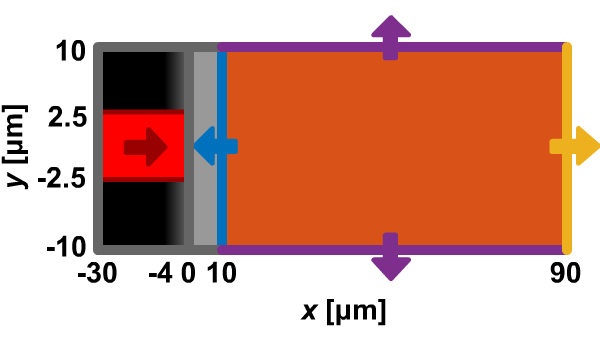
\includegraphics[width=0.6\linewidth]{Figures/tnsa_diagram.png}
\caption{Schematic diagram to show how the end states of particles are characterised, and the path of the laser pulse. We monitor electrons starting in an exponential pre-plasma with $2\text{ }\mu$m scale-length between $x=-4\text{ }\mu$m and $x=0\text{ }\mu$m. Once these electrons pass the rear surface of the solid ($x=10\text{ }\mu$m), they can \textbf{\textcolor{matlabBlue}{reflux}} back into the solid, remain \textbf{\textcolor{matlabOrange}{outside}} the solid but within the simulation window, or escape in the \textbf{\textcolor{matlabYellow}{longitudinal}} or \textbf{\textcolor{matlabPurple}{transverse}} directions.}
\label{fig:tnsa_probe_schematic}
\end{figure}

It was found that $\text{Au}^{51+}$ targets required a greater resolution to suppress self-heating, and so these simulations ran with 5 nm cells and 150 ppc, for 160 fs in a smaller simulation window. This reduced window spanned $-10$ $\mu$m to $10$ $\mu$m in $x$ (pre-plasma $x=-4$ $\mu$m to 0, solid $x=0$ to 2 $\mu$m), and from  $-4$ $\mu$m to $4$ $\mu$m in $y$. The temporal and spatial profiles of the laser pulse remained the same as the C runs.

In our simulations, we used enhanced particle probes which output particle momentum, ID and the time the particle passes the probe. By placing probes at $x = \{-29\text{, }0\text{, }10\text{, }89\}\text{ }\mu$m in C simulations, we could categorise electrons leaving the solid by their four possible end-states, also summarised in Figure \ref{fig:tnsa_probe_schematic}. Electrons could be reflected by the sheath field and reflux back into the target, or could possess enough energy to overcome the sheath field and escape through the $x_\text{max}$ boundary. Electrons could also escape through a $y$-boundary, but this doesn't tell us if they would escape the solid or if they would eventually reflux, so we consider these electrons lost. Finally, electrons could be absorbed into the sheath field, and end the simulation outside the solid region but still within the simulation window. In these characterisation studies, we only track the evolution of electrons which initially started in the pre-plasma ($x<0\text{ }\mu$m), and only after passing the rear target surface for the first time. This is because the electrons may trigger the front probe multiple times on their way into the target, but they won't act like hot electrons until they possess the energy to fully traverse the solid.

The end-state of electrons varied over the run-time of the simulation. In Figure \ref{fig:tnsa_fate_t}, we bin electrons by the time they leave solid through the $10\text{ }\mu$m probe in the C target runs, plotting the number spectrum of outgoing probe hits and colouring this spectrum according to the end-state of particles in each bin. Electrons can be counted more than once if they leave the target again after re-entry.

\begin{figure}
\centering
\begin{subfigure}{.49\textwidth}
  \centering
  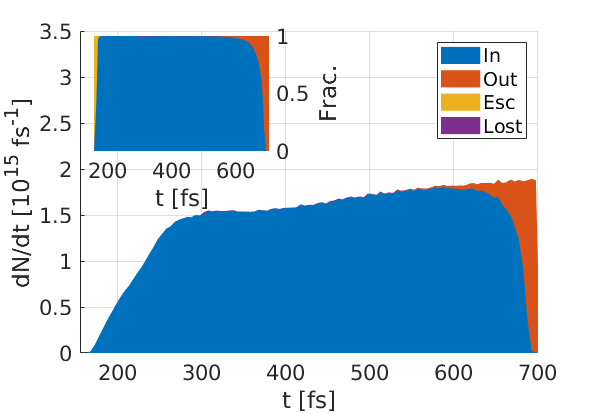
\includegraphics[width=1\linewidth]{Figures/C_1e20_t_r.png}
  \caption{C $10^{20} \text{Wcm}^{-2}$}
\end{subfigure}%
\begin{subfigure}{.49\textwidth}
  \centering
  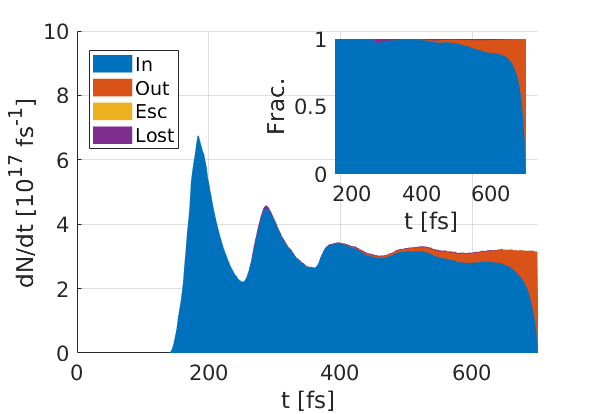
\includegraphics[width=1\linewidth]{Figures/C_1e22_t_r.png}
  \caption{C $10^{22} \text{Wcm}^{-2}$}
\end{subfigure}
\caption{The number spectra of electrons leaving the solid through the rear surface for the two carbon simulations, binned by outgoing time. The plots are coloured to show the proportion of particles in each of the four end-states. A normalised fraction of end-states is provided in the sub-figures to show areas which are under-represented in dN/dt.}
\label{fig:tnsa_fate_t}
\end{figure}

Figure \ref{fig:tnsa_fate_t} shows that most electrons reflux back into the target, and we only see particles escaping through $x_\text{max}$ early in the simulation before a sheath field is established (as seen in the Figure \ref{fig:tnsa_fate_t}a insert for low $t$). While some electrons end the simulation in the background region, this mostly occurs for electrons exiting towards the end of the simulation, suggesting they simply haven't had time to reflux. The lack of lost electrons suggests the transverse simulation window size is sufficient for capturing most electron end-states.

We also inspected the end states of particles after binning by outgoing total momentum, as shown in Figure \ref{fig:tnsa_fate_p}. Again, in both C simulations we find the majority of electrons reflux back into the target, except for the highest energy electrons which escape. We find that it's mostly the lower energy electrons which end the simulation outside the solid, which suggests the higher energy electrons don't spend much time in reflux events.

\begin{figure}
\centering
\begin{subfigure}{.49\textwidth}
  \centering
  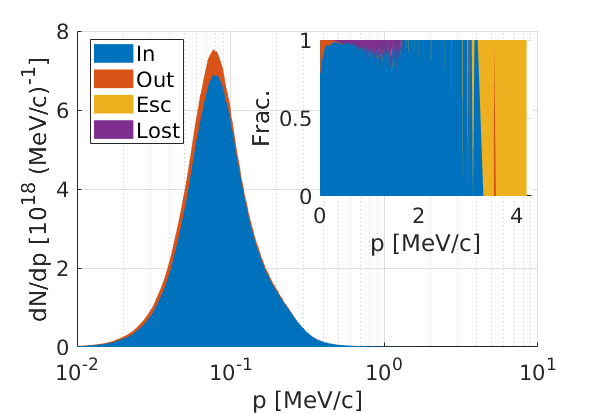
\includegraphics[width=1\linewidth]{Figures/C_1e20_p_r.png}
  \caption{C $10^{20} \text{Wcm}^{-2}$}
\end{subfigure}%
\begin{subfigure}{.49\textwidth}
  \centering
  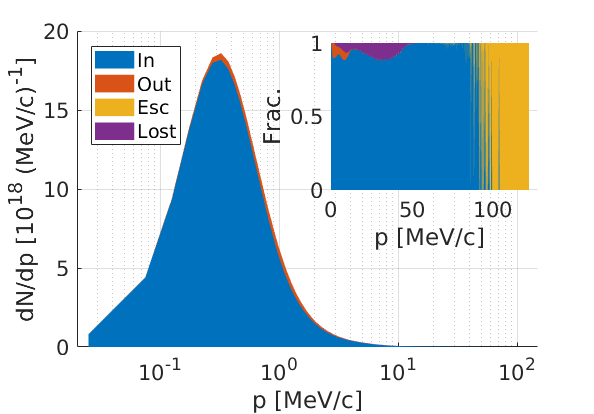
\includegraphics[width=1\linewidth]{Figures/C_1e22_p_r.png}
  \caption{C $10^{22} \text{Wcm}^{-2}$}
\end{subfigure}
\caption{The number spectra of electrons leaving the solid through the rear surface for the two carbon simulations, binned by outgoing total momentum. The plots are coloured to show the proportion of particles in each of the four end-states. A normalised fraction of end-states is provided in the sub-figures to show areas which are under-represented in dN/dp.}
\label{fig:tnsa_fate_p}
\end{figure}

Figures \ref{fig:tnsa_fate_t} and \ref{fig:tnsa_fate_p} confirm that electrons mostly reflux back into the target when escaping through the rear solid boundary, but we can also look at how electron energy changes when refluxing. We binned refluxing electrons by the outgoing $x$-component of momentum on the rear boundary, $p_x^\text{out}$ in all four simulations, and calculated the average value of $|p_x^\text{in}/p_x^\text{out}|$ in each bin. These curves, along with a shaded area to show the variation of the momentum change in each bin, have been shown in Figure \ref{fig:tnsa_loss}.

\begin{figure}
\centering
  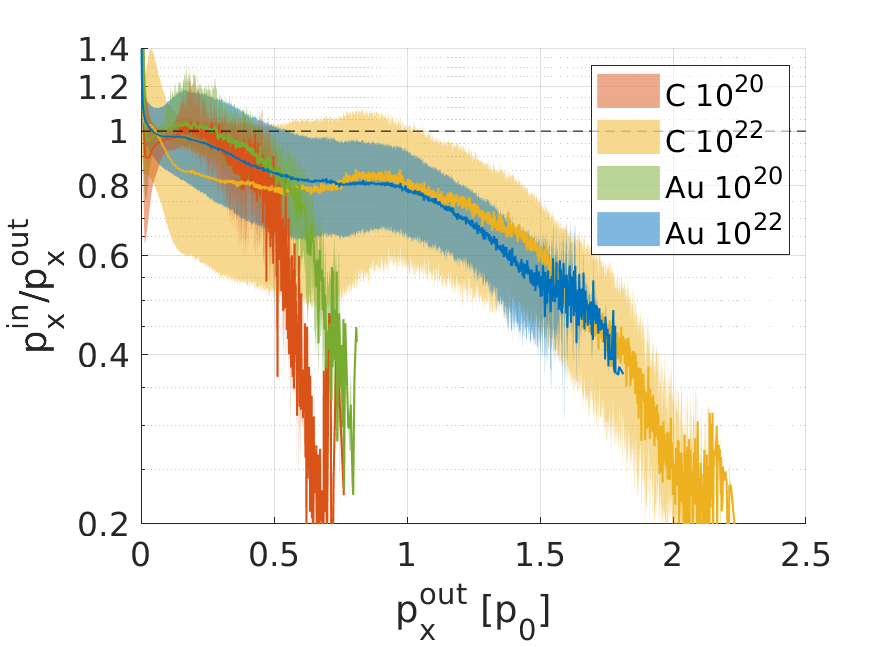
\includegraphics[width=0.6\linewidth]{Figures/tnsa_rear.png}
\caption{The longitudinal momentum loss in a refluxing event on the rear solid surface, binned by outgoing hot electron momentum. The solid line shows the average momentum change in a bin, and the shaded regions represent the average deviation both above and below the solid line. The dotted line represents no change in the momentum magnitude - everything below has lost momentum, everything above has gained it. The outgoing momentum is in units of the ponderomotive momentum $p_0=a_0m_e c$, and simulations are labelled by the target material, and the laser intensity in $\text{Wcm}^{-2}$.}
\label{fig:tnsa_loss}
\end{figure}

We find the momentum loss behaviour is quite similar for targets of different thickness and density, and is qualitatively similar at different laser intensities. The highest energy electrons seem to lose the most energy when refluxing, with the lower energy electrons staying at similar $p_x$ magnitude when returning. However, as seen in Figure \ref{fig:tnsa_fate_p}, the majority of probe-hits occur for these lower energy electrons. It is useful to also look at the total momentum loss in each bin, instead of the average loss per electron.

\begin{figure}
\centering
\begin{subfigure}{.49\textwidth}
  \centering
  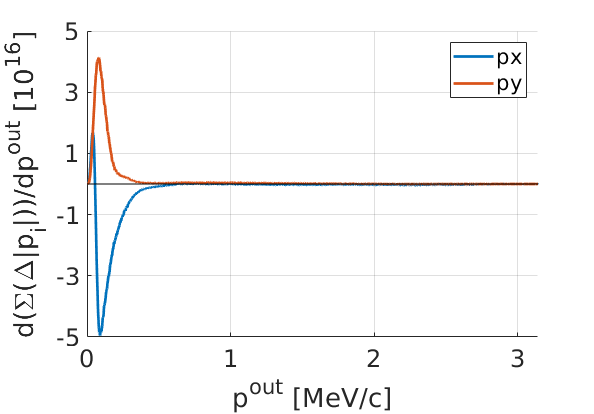
\includegraphics[width=1\linewidth]{Figures/C_1e20_pi_loss.png}
  \caption{C $10^{20} \text{Wcm}^{-2}$}
\end{subfigure}%
\begin{subfigure}{.49\textwidth}
  \centering
  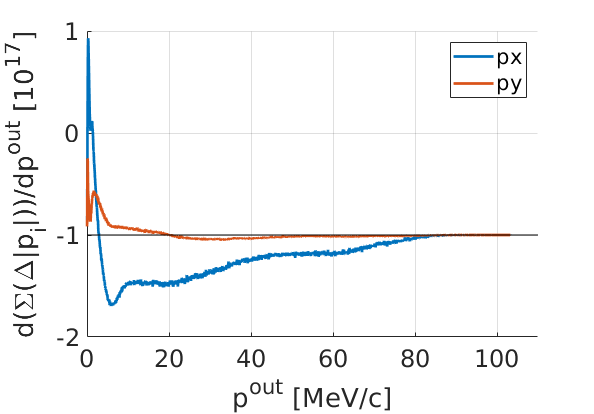
\includegraphics[width=1\linewidth]{Figures/C_1e22_pi_loss.png}
  \caption{C $10^{22} \text{Wcm}^{-2}$}
\end{subfigure}
\caption{Electrons which pass the rear surface of the solid and then re-enter are binned by their outgoing total momentum. The changes in the momentum component magnitude ($|p_i^\text{in}|-|p_i^\text{out}|$) are summed over all electrons in the bin, and plotted for $p_x$ and $p_y$. No $p_z$ change has been plotted, as this remained 0 for all particles in our 2D simulations. }
\label{fig:tnsa_pi_loss}
\end{figure}

After binning all refluxing electrons by outgoing momentum, Figure \ref{fig:tnsa_pi_loss} shows total change of momentum component summed over every electron in each bin. Figure \ref{fig:tnsa_pi_loss}a shows that most of the longitudinal momentum is lost by the lower energy electrons. A loss of longitudinal momentum agrees with observations by Vysko\v{c}il \textit{et al} \cite{bremPIC:Vyskocil}, who suggest the loss would explain the increase in bremsstrahlung emission angle. Our results go further, and suggest that an increased angle can be attributed to both a decrease in $p_x$, and an increase in $p_y$ when refluxing. This relationship is less clear in the higher intensity Figure \ref{fig:tnsa_pi_loss}b, but we still observe a dominant loss in longitudinal momentum and a gain in transverse momentum.

We also note that the gain in $p_y$ is less than the loss in $p_x$, and so on average, electrons lose energy when refluxing. The average loss of total momentum during a reflux event has been calculated for each boundary in each simulation, and is given in Table \ref{table:tnsa_dp}.

\begin{table}[h!]
\centering
\begin{tabular}{l c c c}
\toprule
\multicolumn{1}{c}{Target} & \multicolumn{3}{c}{$\langle\Delta p\rangle$ [keV/c]} \\
 & Front & Rear & Total \\
\midrule
$10^{20} \text{ Wcm}^{-2}$, C & -28.2766 & -3.82309 & -7.46456 \\
$10^{20} \text{ Wcm}^{-2}$, Au & -112.953 & -3.04252 & -6.95298 \\
$10^{22} \text{ Wcm}^{-2}$, C & -159.474 & -196.172 & -180.774 \\
$10^{22} \text{ Wcm}^{-2}$, Au & -139.194 & -141.853 & -141.149 \\
\bottomrule
\end{tabular}
\caption{Mean total momentum changes for all refluxing electrons, broken down into front reflux events (laser and pre-plasma side), rear reflux events (initially solid density to vacuum interface), and all reflux events combined.}
\label{table:tnsa_dp} 
\end{table}

As the momentum components are changing in different ways, the angular spectrum of electrons leaving the solid will be different to the spectrum of electrons coming back in. These spectra are compared for rear boundary refluxing electrons in Figure \ref{fig:tnsa_ang_spectra} for the two C simulations. In Figure \ref{fig:tnsa_ang_spectra}a  we see the angular spectra tending to a more uniform distribution, while we see little change in the total spectrum in the higher intensity Figure \ref{fig:tnsa_ang_spectra}b.

\begin{figure}
\centering
\begin{subfigure}{.49\textwidth}
  \centering
  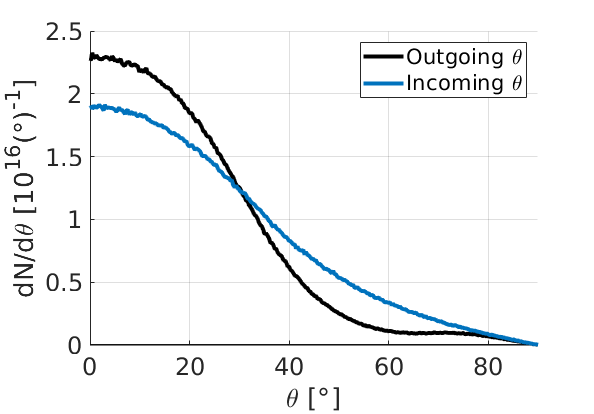
\includegraphics[width=1\linewidth]{Figures/C_1e20_ang_spectra_r.png}
  \caption{C $10^{20} \text{Wcm}^{-2}$}
\end{subfigure}%
\begin{subfigure}{.49\textwidth}
  \centering
  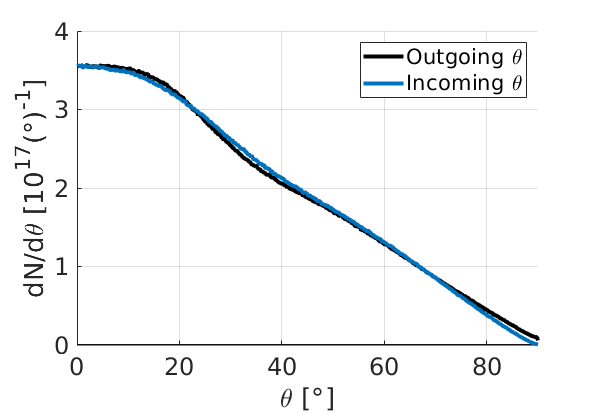
\includegraphics[width=1\linewidth]{Figures/C_1e22_ang_spectra_r.png}
  \caption{C $10^{22} \text{Wcm}^{-2}$}
\end{subfigure}
\caption{Angular distributions of refluxing electrons when escaping the solid target (outgoing) and returning to the solid (incoming).}
\label{fig:tnsa_ang_spectra}
\end{figure}

We can characterise the angular distributions for refluxing electrons further. In Figure \ref{fig:tnsa_theta_change}, we bin refluxing electrons by their outgoing angle, and compare it to their incoming angle. On average, we find that electrons with low $\theta$ typically come back in with a larger angle to the laser axis, and electrons leaving with high $\theta$ come back lower.

\begin{figure}
\centering
  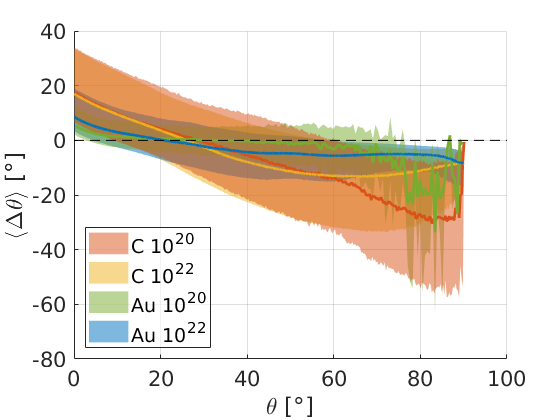
\includegraphics[width=0.6\linewidth]{Figures/theta_change.png}
\caption{Refluxing electrons were binned by their outgoing angle with respect to the laser axis $\theta$ when leaving the solid on either the front or rear surfaces. The mean angle change upon returning to the solid has been calcuated in each bin, and is shown as the solid line for all 4 simulations. The upper and lower shaded regions span up to the average deviation $|\Delta\theta - \langle\Delta\theta\rangle|$ for all electrons above and below $\langle\Delta\theta\rangle$ respectively. }
\label{fig:tnsa_theta_change}
\end{figure}

Despite little change in the Figure \ref{fig:tnsa_ang_spectra}b data, we can see from Figure \ref{fig:tnsa_theta_change} that there is still some scatter when refluxing. As the shaded area of uncertainty remains a similar size for all outgoing $\theta$, this could provide a useful measure in characterising the amount of scatter in a reflux event. The average values of the bin uncertainty range $\sigma_{\langle\Delta\theta\rangle}$, weighted by the number of electrons in each bin, have been provided in Table \ref{table:tnsa_dang}.

\begin{table}[h!]
\centering
\begin{tabular}{l c c c}
\toprule
\multicolumn{1}{c}{Target} & \multicolumn{3}{c}{$\sigma_{\langle\Delta\theta\rangle}$ [$\degree$]} \\
 & Front & Rear & Total \\
\midrule
$10^{20} \text{ Wcm}^{-2}$, C & 27.609 & 25.398 & 27.2838 \\
$10^{20} \text{ Wcm}^{-2}$, Au & 10.2631 & 14.8376 & 10.4962 \\
$10^{22} \text{ Wcm}^{-2}$, C & 27.3305 & 34.8999 & 31.7729 \\
$10^{22} \text{ Wcm}^{-2}$, Au & 15.0984 & 30.796 & 21.7208 \\
\bottomrule
\end{tabular}
\caption{Mean widths of the shaded error region in Figure \ref{fig:tnsa_theta_change}. This mean-width is calculated using an average weighted by the number of electrons in each bin.}
\label{table:tnsa_dang} 
\end{table}

\pagebreak

\section{Code implementation} \label{sec:code}

Section \ref{sec:theory} provides the equations which are used to create the hybrid routines, with references to original sources. This section explores how these equations have been implemented into \texttt{EPOCH}, discussing the new hybrid directory in the source code, and the changes made to pre-existing code files.

The hybrid mode consists of two main changes to \texttt{EPOCH}, the first of which being the hybrid-PIC loop. When running in hybrid mode, instead of changing the main PIC-loop in \textcolor{blue}{epoch$n$d.F90}, we pass control to a second PIC-loop found in \textcolor{blue}{hybrid/hybrid.F90}. This routine is responsible for calling the hybrid subroutines.

Hybrid geometries are specified in the code using a new solid data-type, which stores all the relevant solid parameters. Multiple solids can be defined in the input deck, and compound targets like plastic can be made by spatially overlapping carbon and hydrogen solids.

The following files have been added to \texttt{EPOCH}, and house the hybrid routines:

\begin{itemize}
\item\large{\textcolor{blue}{hybrid/hybrid.F90}} - hybrid PIC loop, initialise, finalise, cold $e^-$ removal
\item\large{\textcolor{blue}{hybrid/hy\_elastic\_davies.F90}} - Davies-style elastic scatter
\item\large{\textcolor{blue}{hybrid/hy\_elastic\_urban.F90}} - Urban-style elastic scatter
\item\large{\textcolor{blue}{hybrid/hy\_fields.F90}} - Hybrid field solver
\item\large{\textcolor{blue}{hybrid/hy\_heating.F90}} - Ohmic and collision heating, ion temperature
\item\large{\textcolor{blue}{hybrid/hy\_ionisation\_loss.F90}} - Ionisation loss and M\o{}ller scatter
\item\large{\textcolor{blue}{hybrid/hy\_laser.F90}} - Laser-based electron injectors
\item\large{\textcolor{blue}{hybrid/hy\_resistivity.F90}} - All resistivity models
\item\large{\textcolor{blue}{hybrid/hy\_shared.F90}} - Interpolation routines
\item\large{\textcolor{blue}{deck/deck\_hy\_laser\_block.F90}} - Input for hybrid electron injectors
\item\large{\textcolor{blue}{deck/deck\_hybrid\_block.F90}} - Switch on/off specific hybrid routines
\item\large{\textcolor{blue}{deck/deck\_solid\_block.F90}} - Define background solids
\end{itemize}

Electron M\o{}ller scatter requires an additional particle variable (\textcolor{blue}{\texttt{optical\_depth\_delta}}), and so to prevent slow-down of MPI routines, the hybrid modules can only be accessed through the \textcolor{blue}{-DHYBRID} preprocessor flag. Sections \ref{sec:code:PIC_loop}-\ref{sec:code:TNSA} discuss the core hybrid routines in more detail.

Additional functionality has been added to \texttt{EPOCH} to allow for characterisation of TNSA boundaries, and to allow injection of hot electrons from the post-processing of PIC codes. Particle probes have been updated to include the ID of particles which trigger them, and also the time a particle passes the probe. The injector block now has the option to inject from file, where momenta, weights, ID, injection time and injection position (for 2D and 3D) are read from different files. These improvements are discussed in sections \ref{sec:code:probes} and \ref{sec:code:file}.

\subsection{Hybrid PIC loop} \label{sec:code:PIC_loop}

The PIC loop in the main \textcolor{blue}{epoch$n$d.F90} file has been positioned inside an IF-statement, which can only be accessed when \textcolor{blue}{\texttt{use\_hybrid}} is false. Otherwise, we call the \texttt{\textcolor{blue}{run\_hybrid\_PIC}} subroutine, which has a similar structure to the standard PIC loop but with a few extra routines. This is shown graphically in the Figure \ref{fig:flowchart_PIC_loop} flow-chart.

\begin{figure}
\centering
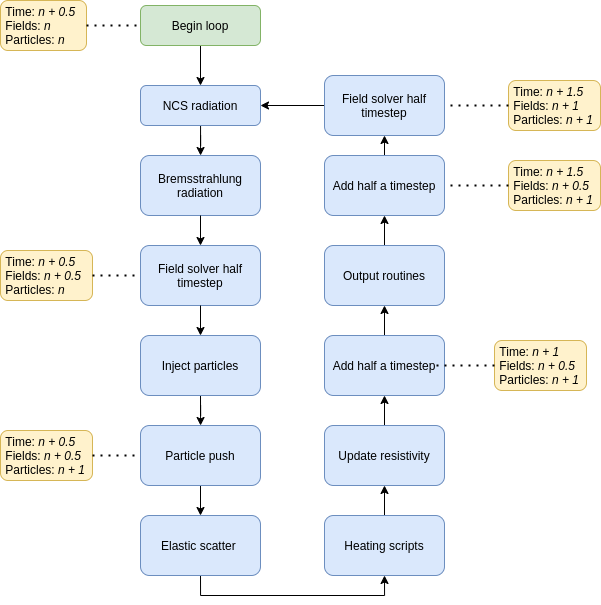
\includegraphics[width=1\linewidth]{Figures/flowchart.png}
\caption{A flow chart which demonstrates the main subroutines called in a hybrid PIC loop. For extra clarity, we also include the current timestep associated with the \texttt{EPOCH} time variable, the fields, and the particle positions. Ionisation loss, Ohmic heating, and thermal equilibration of electron and ion species all fall under the label of ``heating scripts'' in this figure.}
\label{fig:flowchart_PIC_loop}
\end{figure}

As in the normal PIC loop, the field update is split into two halves, such that we have time-centred fields for leap-frogging the particle push. This allows us to use the same particle pusher as in the traditional PIC code, with additional momentum-changing scripts like elastic scatter and ionisation loss occurring separately. 

The loop starts and finishes with \textcolor{blue}{\texttt{time}} evaluated half a timestep ahead of the particles and fields, and we output with fields evaluated half a timestep behind the particles for consistency with the normal PIC loop.

\subsection{Solid type} \label{sec:code:solid}

The hybrid routines describe how electrons pass through solids, which are represented in the code as a new solid type. These are defined in \textcolor{blue}{shared\_data.F90}, which in \texttt{EPOCH3D} reads

\begin{lstlisting}[style=myInputDeck]
  TYPE solid
  
    ! Input variables
    REAL(num) :: Iex = -1.0_num
    REAL(num) :: rad_len = -1.0_num
    REAL(num) :: mass_no = -1.0_num
    INTEGER :: Z = -1
    INTEGER :: res_model = 1
    REAL(num), ALLOCATABLE :: ion_density(:,:,:), el_density(:,:,:)

    ! Derived variables
    REAL(num) :: theta_fac, ln_s, Z_prime
    REAL(num) :: Iex_term, dEdx_C
    REAL(num) :: urb_sig, urb_high, urb_el(22), urb_pos(22)
    REAL(num), ALLOCATABLE :: heat_capacity(:,:,:)
    
  END TYPE solid
\end{lstlisting}

Here, \textcolor{blue}{\texttt{mass\_no}} and \textcolor{blue}{\texttt{Z}} refer to the mass and atomic numbers of the solid respectively. The \textcolor{blue}{\texttt{ion\_density}} array describes the ion number density of the solid in each cell of the simulation window (on the local rank). This value can be set to zero in cells where the solid is not present, allowing the user to control the solid geometries within the simulation window. Here, \textcolor{blue}{\texttt{electron\_density}} corresponds to the total electron number density, and is always set to the product of the solid's ion number density and the atomic number (does not change with ionisation state).

While individual solid types refer to a single elemental material, compound targets can be created by spatially overlapping solids. For example, plastic could be made by defining a carbon solid and a hydrogen solid in the same cells, with the ion densities of each solid summing to the ion density of the plastic as a whole. The \textcolor{blue}{\texttt{Iex}} and \textcolor{blue}{\texttt{rad\_len}} variables denote the mean excitation energy (ionisation loss variable) and radiation length (Urban scatter variable) of the material as a whole. This means in the case of plastic, \textcolor{blue}{\texttt{Iex}} should be set to the mean excitation energy of plastic in both the carbon and hydrogen solids, and not the individual mean excitation energies of carbon and hydrogen respectively. The code uses the mean excitation energy corresponding to the solid with the largest electron number density in that cell.

There are currently 4 resistivity models available in the hybrid code, and different solids can use different resistivities. When updating the resistivity, the code looks for the solid with the highest electron number density in the cell, and uses the \textcolor{blue}{\texttt{res\_model}} variable of that solid to pick which resistivity model to use. This way, multiple resistivity models can be used in the same simulation.

The remaining variables are derived quantities used to speed up the ionisation, elastic scatter, and heating routines:
%
\begin{itemize}
\item \textcolor{blue}{\texttt{theta\_fac}} $= Ze^4/(2\pi\epsilon_0^2)$
\item \textcolor{blue}{\texttt{ln\_s}} $=4\epsilon_0 h / (Z^{1/3}m_e e^2)$
\item \textcolor{blue}{\texttt{Z\_prime}} $ = Z^{-4/3}k_B/e$
\item \textcolor{blue}{\texttt{Iex\_term}} $= 2m_e^2c^4/{I_{ex}}^2$
\item \textcolor{blue}{\texttt{dEdx\_C}} $= 1 + 2\ln\left(I_{ex}\sqrt{\epsilon_0 m_e}/(\hbar e)\right)$
\item \textcolor{blue}{\texttt{urb\_sig}} is the elastic cross section interpolated to $Z$ for the current solid
\item \textcolor{blue}{\texttt{urb\_high}} is a high energy correction interpolated to $Z$ for the current solid
\item \textcolor{blue}{\texttt{urb\_el(22)}} is a $\lambda_1(\epsilon_k)$ table for electrons 
\item \textcolor{blue}{\texttt{urb\_pos(22)}} is a $\lambda_1(\epsilon_k)$ table for positrons
\item \textcolor{blue}{\texttt{heat\_capacity}} is the heat capacity of the solid
\end{itemize}
%
where we have used the same notation as in the theory sections where these concepts are introduced.

\texttt{EPOCH} stores solids in the \textcolor{blue}{\texttt{solid\_array}}, and stores the number of solids in the \textcolor{blue}{\texttt{solid\_count}} variable.

\subsection{Hybrid injectors} \label{sec:code:injector}

The equations in Section \ref{sec:theory:inject} describe how many electrons we may expect to inject in a given timestep, but the implementation in the code provides more flexibility than outlined in that section. These injection routines use the new \textcolor{blue}{\texttt{hy\_laser\_block}} data type, and the syntax is a combination of the laser routines and the injection routines.

In \texttt{EPOCH3D}, the hybrid laser block has the following form:

\begin{lstlisting}[style=myInputDeck]
  TYPE hy_laser_block

    ! Similar syntax to the laser_block type, but without phase
    INTEGER :: boundary
    INTEGER :: ppc

    ! Only spatial profile can vary spatially
    REAL(num), DIMENSION(:,:), POINTER :: profile

    LOGICAL :: use_time_function, use_profile_function
    LOGICAL :: use_omega_function
    TYPE(primitive_stack) :: time_function, profile_function
    TYPE(primitive_stack) :: omega_function

    REAL(num) :: intensity, omega, t_start, t_end, profile_min 
    REAL(num) :: efficiency
    INTEGER :: omega_func_type, species
    LOGICAL :: has_t_end

    INTEGER :: mean, e_dist, ang_dist

    ! User specified energy/weight values
    REAL(num) :: user_mean_KE, user_weight
    REAL(num) :: las_weight_KE
    LOGICAL :: ignore_las

    ! Angular distribution variables
    REAL(num) :: user_theta_max, cos_n_power, top_hat_L
    REAL(num) :: sheng_angle, mean_mult
    REAL(num) :: theta_mean, phi_mean
    LOGICAL :: use_moore_max
    LOGICAL :: use_sheng_dir

    TYPE(hy_laser_block), POINTER :: next

  END TYPE hy_laser_block
\end{lstlisting}

where many variables are analogous to those found in the laser block and injector block types. This allows the user to describe a laser in the input deck in much the same way as a normal laser (with spatially varying profile, peak intensity, wavelength and temporal envelope), and to also describe the number of macro-particles to be injected using these laser parameters.

This block allows the user to choose between multiple models for the mean electron energy, energy distribution and angular distribution, as discussed in the following subsections.

\subsubsection{Mean energy}

There are three options for calculating the mean electron energy, $\langle\epsilon\rangle$ from the laser intensity, $I$ and wavelength, $\lambda$ currently present in the boundary cell:
%
\begin{itemize}
  \item \textcolor{blue}{\texttt{a0}}: $\langle\epsilon\rangle = a_0 m_e c^2$, see (\ref{eq:full_a0}) 
  \item \textcolor{blue}{\texttt{wilks}}: $\langle\epsilon\rangle = 
      \left(
         \sqrt{1 + \frac{I\lambda^2}{1.37\times10^{18} Wcm^{-2}\mu m^2 }}
         - 1 
      \right) m_e c^2$, see \cite{theory:Wilks}
  \item \textcolor{blue}{\texttt{e\_val}}: User-defined mean energy. 
\end{itemize}
%
In the case of \textcolor{blue}{\texttt{e\_val}}, the laser properties are not used to calculate the mean energy (although they may still be used to determine how many particles must be injected). Instead, this user defined mean energy is stored in the \textcolor{blue}{\texttt{user\_mean\_KE}} variable in the hybrid laser block. The choice of mean energy is stored in the \textcolor{blue}{\texttt{mean}} hybrid laser block variable.

\subsubsection{Energy distribution} \label{sec:code:injector:energy}

The hybrid laser block is capable of injecting electrons according to one of six energy distribution functions. While there are only three unique energy distributions (\textcolor{blue}{\texttt{mono}}, \textcolor{blue}{\texttt{exp}} and \textcolor{blue}{\texttt{top\_hat}}), these distributions can be achieved using different macro-particle weighting methods. The possible energy distributions allowed by the code are characterised by the mean electron energy $\langle\epsilon\rangle$, and can be summarised as:

\begin{itemize}
  \item \textcolor{blue}{\texttt{mono}}: All electron energies set to $\langle\epsilon\rangle$, and the total number of electrons to inject in this cell and timestep (\ref{eq:inject_no}) is split equally between the injected macro-particle weights.
%
  \item \textcolor{blue}{\texttt{exp}}: Macro-particle energies assigned using an exponential probability density function (PDF), $P(\epsilon)$, 
  \begin{align} \label{eq:exp_dist}
    P(\epsilon) = \frac{1}{\langle\epsilon\rangle} e^{-\epsilon/{\langle\epsilon\rangle}}
  \end{align}
where all macro-particle weights are equal, and sum to the total number of particles to inject in this cell and timestep according to (\ref{eq:inject_no}).
% 
  \item \textcolor{blue}{\texttt{top\_hat}}: Macro-particle energies are assigned from a uniform distribution between limits $(1-L)\langle\epsilon\rangle$ and $(1+L)\langle\epsilon\rangle$, where the fractional width, $0<L\leq 1$ is defined by the user and stored in the \textcolor{blue}{\texttt{top\_hat\_L}} variable in the hybrid laser block. The total number of electrons to inject in this cell and timestep (\ref{eq:inject_no}) is split equally between the injected macro-particle weights.
% 
  \item \textcolor{blue}{\texttt{exp\_weight}}: Macro-particle energies are assigned from a uniform distribution between limits 0 and $M\langle\epsilon\rangle$, where the factor, $M$, is defined by the user and stored in the \textcolor{blue}{\texttt{mean\_mult}} variable in the hybrid laser block. The weights of all injected macro-particles are exponentially distributed, such that the probability density function of injected real particles matches (\ref{eq:exp_dist}), and the weights sum to the total number to be injected (\ref{eq:inject_no}). This distribution is useful if you are interested in the behaviour of high energy electrons from an exponential distribution, as the \textcolor{blue}{\texttt{exp}} distribution may create too many low energy macro-electrons to get good high energy statistics.
%
  \item \textcolor{blue}{\texttt{mono\_weight}}: Macro-particle energies are set to $\langle\epsilon\rangle$, and particle weights are set to a user-defined value stored in the hybrid laser block variable \textcolor{blue}{\texttt{user\_weight}}. Useful for particle beams or bunches.
%
  \item \textcolor{blue}{\texttt{mono\_las\_weight}}: The total number of electrons to inject in this cell and timestep is calculated from the laser parameters (\ref{eq:inject_no}), and is split equally between the injected macro-particle weights. In this model, the energies assigned to the macro-particles can be different to the $\langle\epsilon\rangle$ value used in calculating the macro-particle weights, and instead takes the user-defined value stored in \textcolor{blue}{\texttt{las\_weight\_KE}}. This is useful if you want to inject a low energy beam with the same weight distribution as the electron injection, in case you wish to ensure the total charge in the simulation window remains neutral.
  
\end{itemize}

Where appropriate, sampling of these distributions is achieved by converting the probability density function $P(\epsilon)$ to a cumulative distribution function $F(\epsilon)$, using
%
\begin{align} \label{eq:CDF}
  F(\epsilon) = \int_{-\infty}^\epsilon P(\epsilon')d\epsilon'
\end{align}
%
where $F(\epsilon)$ ranges between 0 and 1. Once an expression for $F(\epsilon)$ is obtained, we rearrange this equation to find an expression for $\epsilon$, and replace the CDF with a random number drawn from a uniform distribution between 0 and 1, $x_r$. The sampling equations are given in Table \ref{table:energy_sample}.

\begin{table}[h!]
\centering
\begin{tabular}{l l}
  \toprule
  Distribution & Energy sampling \\
  \midrule 
  \textcolor{blue}{\texttt{exp}} & $\epsilon = -\langle\epsilon\rangle\ln(1-x_r)$ \\
  \textcolor{blue}{\texttt{top\_hat}} & $\epsilon = L\left(x_r-\frac{1}{2}\right) + \langle\epsilon\rangle$ \\
  \textcolor{blue}{\texttt{exp\_weight}} & $\epsilon = Mx_r\langle\epsilon\rangle$ \\
  \bottomrule
\end{tabular}
  \caption{Equations used to sample energies in the non-uniform energy distributions for the hybrid electron injector. Here, $x_r$ refers to a uniformly distributed random number between 0 and 1, and distribution-specific parameters are defined in Section \ref{sec:code:injector:energy}.}
\label{table:energy_sample} 
\end{table}
%
The choice of energy distribution model is stored in the \textcolor{blue}{\texttt{e\_dist}} hybrid laser block variable. The \textcolor{blue}{\texttt{ignore\_las}} variable is used to prevent the laser parameters being calculated when running with a \textcolor{blue}{\texttt{mono\_weight}} distribution.

\subsubsection{Angular distribution} \label{sec:code:injector:angles}

Once the weights and energies of the macro particles have been sampled, we must determine the momentum direction of the incoming particles. In Section \ref{sec:theory:inject}, we introduce the Moore angle for injection cone widths (\ref{eq:Moore}) and the Sheng angle for the cone axis in oblique laser-solid collisions (\ref{eq:Sheng}). Both of these energy-dependent injection characteristics can be turned on and off using the hybrid laser block variables \textcolor{blue}{\texttt{use\_moore\_max}} and \textcolor{blue}{\texttt{use\_sheng\_dir}}.

The basic form of injection is into a cone, where the half angle, $\theta_{\text{max}}$ is taken to be the smaller of the Moore angle (if used), or a user-defined cone angle stored in the \textcolor{blue}{\texttt{user\_theta\_max}} hybrid laser block variable. Within this cone, we sample $\theta$ values using one the following distributions:

\begin{itemize}
  \item \textcolor{blue}{\texttt{uniform}}: Electron directions are uniformly distributed within the cone, which corresponds to a probability density function for solid angles $P(\Omega)$ of the form:
  \begin{align}
    P(\Omega) = \frac{1}{2\pi(1-\cos\theta_{max})}
  \end{align} 
% 
  \item \textcolor{blue}{\texttt{cos}}: Electrons are injected to a cone of maximum cone half-angle $\theta_{\text{max}}$, in a distribution proportional to $\cos^n(\theta)$, where $n$ is a user defined parameter stored in the \textcolor{blue}{\texttt{cos\_n\_power}} hybrid laser block variable. The corresponding PDF is:
   \begin{align}
    P(\Omega) = \frac{n+1}{2\pi\left(1 - \cos^{n+1}(\theta_\text{max})\right)}\cos^{n}(\theta),
  \end{align}
where we note this returns the uniform case for $n=0$.
% 
  \item \textcolor{blue}{\texttt{beam}}: All $\theta$ values are set to zero, particles are injected in a straight line perpendicular to the boundary.
\end{itemize}

The choice of angular distribution model is stored in the \textcolor{blue}{\texttt{ang\_dist}} hybrid laser block variable. In all models, the azimuthal angle $\phi$ is sampled uniformly. As in Section \ref{sec:code:injector:energy}, we can sample from these PDFs by converting them into CDFs, and replacing the CDF with a random number. These functions are given in Table \ref{table:angular_sample}

\begin{table}[h!]
\centering
\begin{tabular}{l l}
  \toprule 
  Distribution & Angular sampling \\
  \midrule 
  \textcolor{blue}{\texttt{uniform}} & $\theta = \cos^{-1}\left(1 - x_r(1-\cos\theta_\text{max})\right)$ \\
  \textcolor{blue}{\texttt{cos}} & $\theta = \cos^{-1}\left((1-x_r(1-\cos^{n+1}\left(\theta_\text{max}\right)))^{\frac{1}{n+1}}\right)$ \\
  \bottomrule
\end{tabular}
  \caption{Equations used to sample $\theta$ values in the non-beam angular distributions for the hybrid electron injector. Here , $x_r$ refers to a uniformly distributed random number between 0 and 1, and distribution-specific parameters are defined in Section \ref{sec:code:injector:angles}.}
\label{table:angular_sample} 
\end{table}

After the code has calculated the $\theta_\text{max}$ value, sampled a $\theta$, $\phi$ direction, and applied a Sheng rotation (if used), the user can perform a final rotation to the injector as a whole using the user-defined ($\theta$, $\phi$) values stored in the hybrid laser block variables \textcolor{blue}{\texttt{theta\_mean}} and \textcolor{blue}{\texttt{phi\_mean}}.

\subsection{Ionisation loss and M\o{}ller scatter} \label{sec:code:ionisation}

As discussed in Section \ref{sec:theory:coll}, ionisation energy loss treatment can be split between a continuous energy loss due to the creation of low energy $\delta$-rays, and discrete emission considering the recoil due to high energy $\delta$-rays. Both approaches are present in the file \textcolor{blue}{\textit{hy\_ionisation\_loss.F90}}, and are accessed through the subroutine \textcolor{blue}{\texttt{run\_ionisation\_loss}}. This subroutine cycles over all species, and calls the continuous and discrete loss subroutines for every particle in an electron species.

The \textcolor{blue}{\texttt{continuous\_energy\_loss}} subroutine calculates the density correction (\ref{eq:theory:density_effect}), then calculates the energy loss, $d\epsilon$ from the stopping power (\ref{eq:ionisation:cont_stopping_power}) and the step size. After applying this loss, $d\epsilon$, the subroutine also outputs $d\epsilon$ for use in the heating routines.

Just as in bremsstrahlung and NCS emission, high energy $\delta$-rays are emitted according to an optical depth model, which requires an additional variable for the \textcolor{blue}{\texttt{particle}} type: \textcolor{blue}{\texttt{optical\_depth\_delta}}. As this could affect the speed of the particle pusher as particles pass between boundaries, all hybrid routines have been hidden behind a pre-compiler flag. This optical depth has also been made a restart variable. At the start of the simulation and after each emission, the hot electrons are assigned an optical depth for emission, $\tau$ from an exponential distribution. After each time step, $\Delta t$, the particle advances an optical distance $\Delta\tau$,
%
\begin{align}
  \Delta\tau = \sigma n_e\Delta t
\end{align}
%
where $\sigma$ is the cross section for high energy $\delta$-ray emission (\ref{eq:ionisation:cross_sec}), and $n_e$ is the background total electron density evaluated at the hot electron position.

\subsection{Heating routines} \label{sec:code:heating}

The original Davies method of heating in a hybrid PIC code uses the heat capacity (\ref{eq:theory:heatCap}), and the heating equations of Ohmic (\ref{eq:theory:heat:Ohmic}) and collisional (\ref{eq:theory:heat:coll}) heating \cite{hybrid:Davies:2002}. When applied to compound targets, the Davies method used a target-averaged atomic number, $Z$. However, as the bremsstrahlung cross section scales with $Z^2$, a compound target and an averaged-$Z$ target would lead to different simulated bremsstrahlung spectra. To fix this, we have extended the Davies model to consider the heating of multiple targets in the same PIC cells.

The heat capacity of each solid is worked out independently using (\ref{eq:theory:heatCap}), and stored in the solid-type variable \textcolor{blue}{\texttt{heat\_capacity}}. To reconcile the different solid heat capacities with the need for a single background temperature in each cell, we introduce an effective heat capacity term, $C_\text{eff}$
%
\begin{align}
  C_\text{eff} = \sum_\text{sol}\left(\frac{Z^{\text{sol}}n_i^{\text{sol}}}{C^{\text{sol}}}\right)
\end{align}
%
where we sum over each solid (sol) present in a given cell. Here, $Z^{\text{sol}}$, $n_i^\text{sol}$ and $C^{\text{sol}}$ refers to the atomic number, ion number density and heat capacity of a solid type respectively. As the heat capacity changes with temperature, the effective heat capacity must be recalculated each step. This variable can be used to obtain the solid-averaged inverse heat capacity
%
\begin{align} 
  \langle\frac{1}{C}\rangle_\text{sol} = \frac{C_\text{eff}}{\sum_\text{sol}\left(Z^{\text{sol}}n_i^{\text{sol}}\right)} = \frac{C_\text{eff}}{n_e^\text{tot}}
\end{align}
%
where we have written the total electron number density in the cell as $n_e^\text{tot}$ for conciseness. Hence, the Ohmic and collisional heating equations for compound targets may be written as
%
\begin{align}
  \Delta T_e =& \frac{\textbf{j}\cdot\textbf{j}\eta dt}{(n_e^\text{tot})^2k_B}C_\text{eff} \\
  \Delta T_e =& \frac{\Sigma_h \Delta \epsilon_h}{(n_e^\text{tot})^2V_{cell}k_B}C_\text{eff}
\end{align}
%
using the same notation as Section \ref{sec:theory:heat}.

\subsection{Field solver} \label{sec:code:fields}

Scipts relating to the hybrid field solver are found in \textcolor{blue}{\texttt{hy\_fields.F90}}. Discretisation of the hybrid field equations (\ref{eq:field:E} - \ref{eq:field:B}) can be achieved in a similar way to the traditional PIC field solver. The step is performed in two half-steps, but with a simple first-order step for the electric field. In 3D, the update for the $x$-component of the magnetic field in a given cell, $B_x^{n+1/2}(i_x,i_y,i_z)$ reads:
%
\begin{equation} \label{eq:code:B}
\begin{aligned}
  B_x^{n+1/2}(i_x,i_y,i_z) = B_x^{n}(i_x,i_y,i_z) - \frac{\Delta t}{2\Delta y}\left(E_z^n(i_x,i_y+1,i_z) - E_z^n(i_x,i_y,i_z)\right) \\ + \frac{\Delta t}{2\Delta z}\left(E_y^n(i_x,i_y,i_z+1) - E_y^n(i_x,i_y,i_z)\right)
\end{aligned}
\end{equation}
%
where $\Delta t$ denotes the timestep, $n$ denotes the time index, and $\Delta y$, $\Delta z$ are the cell sizes in the $y$ and $z$ directions. The hybrid field solver is only a first order method, as the electric fields are simply recalculated at the $B$ timestep after $B$ has been updated, via
%
\begin{equation} \label{eq:code:E}
\begin{aligned}
  E_x^{n+1/2}(i_x,i_y,i_z) &= \frac{1}{2}\left(\eta(i_x+1,i_y,i_z) + \eta(i_x,i_y,i_z)\right) \\ 
  &\left[\frac{1}{\mu_0\Delta y} \left(B_z^{n+1/2}(i_x,i_y+1,i_z) - B_z^{n+1/2}(i_x,i_y,i_z)\right)\right.\\
  &- \frac{1}{\mu_0 \Delta z} \left(B_y^{n+1/2}(i_x,i_y,i_z+1) - B_y^{n+1/2}(i_x,i_y,i_z)\right) \\
  &- J_x(i_x,i_y,i_z)]
\end{aligned}
\end{equation}
%
where we note that the resistivity, $\eta$ is a cell-centred variable, and the current density, $\textbf{J}$ shares the same stagger as the electric field. The resistivity and current density in (\ref{eq:code:E}) are evaluated at different times relative to the $B$ in the two half steps, and could be written as $\eta^{n}$, $J_x^{n}$ for the update after \textit{Bremsstrahlung radiation}, and $\eta^{n+1/2}$, $J_x^{n+1/2}$ for the update before \textit{NCS radiation} (see Figure \ref{fig:flowchart_PIC_loop}). Currently, there is no purpose to splitting up the field update before and after radiation - but I believe these field updates could be moved around such that the output routines print fields evaluated at the same time as the particle positions (see discussion of issue \#2229, \texttt{EPOCH GitLab}). I will therefore leave the field update in two halves to allow for a quick fix in case the main PIC loop is updated.

\begin{figure}
\centering
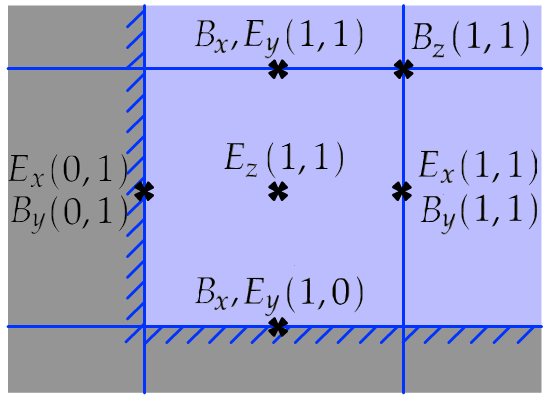
\includegraphics[width=0.6\linewidth]{Figures/Cell_stagger.png}
\caption{Visualisation of field staggering in an \texttt{EPOCH2D} simulation. Here we show how the fields are arranged on the $x_\text{min}$, $y_\text{min}$ simulation window corner, and fields are labelled by their cell indices. The greyed out cells denote ghost cells, starting at index 0.}
\label{fig:cell_stagger}
\end{figure}

We must also consider the boundary conditions of our new field solver. The distribution of field evaluation points on the staggered grid has been shown for a 2D grid in Figure \ref{fig:cell_stagger}. The field point $E_z(1,1)$ depends on the neighbouring values $B_y(1,1)$, $B_x(1,1)$, and also ghost cell field points $B_x(1,0)$ and $B_y(0,1)$. If these ghost cell points were set to match their closest simulation-cell counterparts, the gradient across $E_z(1,1)$ would always be zero, and no magnetic field could contribute to the electric field in this point. To correct for this, we update all cells from indices \textcolor{blue}{\texttt{0}} to \textcolor{blue}{\texttt{nx+1}} (for $x$). We then apply zero-curl boundary conditions to cells which are not directly involved in the calculation of simulation window fields, as performed by the \textcolor{blue}{\texttt{field\_zero\_curl}} subroutine. This boundary condition sets the values of ghost cells to match the first ghost cell, for example, $E_x(-1,1)$, $E_x(-2,1)$, ... $E_x(1-ng,1)$ would be set to $E_x(0,1)$, where \textcolor{blue}{\texttt{ng}} is the number of ghost cells.

\subsection{Resistivity models} \label{sec:code:res}

In Section \ref{sec:theory:resistivity}, we introduce the Lee-More resistivity model for cold dense solids (\ref{eq:LeeMore}). The full model relies on the chemical potential (\ref{eq:chem_pot}), but this relies on a computationally costly evaluation of an inverse polylogarithm function for each cell in each timestep, which would be a significant bottleneck for the code. Instead, we use a reduced form of the Lee-More model which avoids the calculation of $\mu$, as done in the hybrid code \texttt{ZEPHYROS} which is discussed in Section \ref{sec:code:res:rlm}.

The resistivity models used by Davies \cite{hybrid:Davies:2002} are also present in the code, including a fit to experimental data for aluminium (Section \ref{sec:code:res:Milch}), and a heuristic model resistivity model for plastic (Section \ref{sec:code:res:plastic}).

\subsubsection{Reduced Lee-More model} \label{sec:code:res:rlm}

In (\ref{eq:LeeMore}), the only terms which depend on the chemical potential are the electron relaxation time $\tau$ (\ref{eq:tau_plas}), and the $A^\alpha$ factor (\ref{eq:A_alpha}). The original Lee-More paper \cite{eta:LeeMore} quotes these terms in the non-degenerate plasma limit $\mu\rightarrow - \infty$,
%
\begin{align}
  A^{\alpha} &\rightarrow \frac{32}{3\pi} \\
  \tau &\rightarrow \frac{12\pi^2\epsilon_0^2}{e^4}\sqrt{\frac{m_e}{2\pi}}\frac{(k_bT_e)^{3/2}}{(Z^*)^2n_i\ln\Lambda}   
\end{align}
%
which are the SI equivalents of the paper's (27 \cite{eta:LeeMore}) and (28a \cite{eta:LeeMore}) respectively, and the terms have the same meaning as in Section \ref{sec:theory:resistivity}. The Lee-More paper also provides a low temperature relaxation time, $\tau_\text{cold}$ given by (\ref{eq:tau_cold}). 

Our \texttt{ZEPHYROS}-style reduced Lee More model starts with an effective hot electron relaxation time, $\tau_\text{hot} = A^{\alpha}\tau$ evaluated in the non-degenerate limit. As the temperature falls, $\tau_\text{hot}$ becomes unphysically small and we switch to an effective cold relaxation time, $\tau_\text{cold}$
%
\begin{align}
  \tau_\text{cold} = \lambda_1 \frac{R_0}{\bar{v}}
\end{align}
%
which is the low temperature relaxation time (\ref{eq:tau_cold}) with an additional fitting parameter, $\lambda_1$. Our reduced Lee-More resistivity formula reads
%
\begin{align}
  \eta &= \frac{m_e}{Z^*n_i e^2 \tau_\text{eff}} \lambda_2 \\
  \tau_\text{eff} &= \max(\tau_\text{hot}, \tau_\text{cold})
\end{align}
%
where $\lambda_2$ is a second fitting parameter for scaling the total resistivity.

\subsubsection{Milchberg fit} \label{sec:code:res:Milch}

In the original Davies code \cite{hybrid:Davies:2002}, the authors use a simpler form for the resistivity, $\eta$ as a function of electron temperature, $T_e$. This comes to a fit from data in an experiment ran by Milchberg \textit{et al} \cite{eta:Al:Milchberg}, which looked at the resistivity of aluminium up to a temperature of 100 eV. The functional form of the Milchberg fit is
%
\begin{align}
  \eta = \frac{T_{e,eV}}{5\times 10^6 + 170 {T_{e,eV}}^{5/2} + 3\times 10^5 T_{e,eV}}
\end{align}
%
where $T_{e,eV}$ is the electron temperature measured in eV.

\subsubsection{Heuristic plastic model} \label{sec:code:res:plastic}

Davies \textit{et al} also derive a heuristic resistivity model for plastic \cite{eta:Davies}, which varies between a saturation resistivity, $\eta_0$, and the Spitzer resistivity. In this paper, Davies explains that while the room-temperature resistivity of an insulator is significantly higher than a conductor, the ionisation brought on by heating enables hot insulators to take on similar charge-carrying characteristics to conductors.

In Boltzmann theory, resistivity, $\eta$ rises linearly with electron temperature, $T_e$ - but this breaks down at a certain $T_e$ value and $\eta$ starts to rise slower than $T_e$. The saturation resistivity refers to the $\eta$ value at this regime change \cite{eta:saturation:Gunnarsson}, and can be roughly described by the Ioffe-Regel criteria
%
\begin{align}
  \eta_0 = \left(\frac{3\pi^2}{n_\text{con}^2}\right)^{1/3}\frac{\hbar e^2}{d}
\end{align}
%
where $n_\text{con}$ is the number density of conduction electrons, and $d$ is the interatomic spacing. In the case of plastic, Davies \textit{et al} assumes $n_e \sim 10^{29} \text{ m}^{-3}$, and quotes $\eta_0 = 2.3\times 10^{-6} \text{ }\Omega \text{m}$.

The parallel Spitzer resistivity, $\eta^\text{Spitzer}_\parallel$ is derived as a correction to the resistivity of an idealised Lorentz gas \cite{eta:Spitzer:Spitzer}, which translated to SI units reads
%
\begin{align}
  \eta^\text{Spitzer}_\parallel = \frac{\pi^{3/2}m_e^{1/2}Z^* e^2 c^4 \ln\Lambda}{2(2k_BT_{e})^{3/2}}\frac{10^{-14}}{\gamma_e(Z^*)}
\end{align}
%
where $\gamma_e$ is a correction factor which has tabulated values in the reference. The perpendicular Spitzer resistivity, $\eta^\text{Spitzer}_\perp$ can be expressed as $\eta^\text{Spitzer}_\perp=\eta^\text{Spitzer}_\parallel F(Z^*)$, where $F(Z^*)$ values are tabulated in Table 1 of a paper by Braginskii, \cite{eta:Spitzer:Braginskii}, which can be approximated to the fit
%
\begin{align}
  F(Z^*) = \frac{1 + 1.198Z^* + 0.222(Z^*)^2}{1 + 2.966Z^* + 0.753(Z^*)^2}
\end{align}
%
by Kuritsyn \textit{et al} \cite{eta:Spitzer:Kuritsyn}. The Davies heuristic model uses the parallel Spitzer resistivity with $Z^*=1$ for plastic, where $\gamma_e = 0.582$ and $F(Z)=1.96$, such that
%
\begin{align}
  \eta_\perp^\text{Spitzer} \approx 1.04\times 10^{-4} \ln\Lambda {T_{e,eV}}^{-3/2}
\end{align}
%
where $T_{e,eV}$ is the electron temperature evaluated in eV. For plastic, Davies uses $\ln\Lambda = 7.7$ such that the full heuristic plastic resistivity model reads
%
\begin{align}
  \eta = \frac{1}{4.3\times 10^5 + 1.3\times 10^3 T_{e,eV}^{3/2}}
\end{align}
%
which tends towards the saturation resistivity at low temperature, and the Spitzer resistivity at high temperature.

\subsection{TNSA boundaries} \label{sec:code:TNSA}

We have implemented simple algorithms to roughly approximate refluxing behaviour, guided by observations in Section \ref{sec:theory:TNSA}. These algorithms can be accessed using a new \textcolor{blue}{\texttt{tnsa}} boundary type in the boundaries block. Our parametrisation takes the form of three key parameters:
%
\begin{itemize}
  \item \textcolor{blue}{\texttt{tnsa\_escape\_KE}}: Above this kinetic energy, all electrons escape (to reproduce particle fates observed in Figure \ref{fig:tnsa_fate_p}).
%
  \item \textcolor{blue}{\texttt{tnsa\_p\_loss}}: Upon refluxing, this value is subtracted from the total momentum magnitude, without changing the momentum direction. Typical values can be taken from Table \ref{table:tnsa_dp}.
% 
  \item \textcolor{blue}{\texttt{tnsa\_scatter\_angle}}: If refluxing with an outgoing polar angle $\theta$, the electron returns with polar angle $\theta + \theta_r$, where $\theta_r$ is a random scatter angle drawn from a uniform distribution between $\pm 0.5 \times \text{\textcolor{blue}{\texttt{tnsa\_scatter\_angle}}}$. This is to reproduce the large scatter uncertainty present in Figure \ref{fig:tnsa_theta_change}, and typical values are given in Table \ref{table:tnsa_dang}.
%
\end{itemize}
%
which are set by the user in the input deck boundary block.

The \textcolor{blue}{\texttt{tnsa}} boundary type behaves the same as the \textcolor{blue}{\texttt{reflect}} boundary type, until the \textcolor{blue}{\texttt{particle\_bcs}} subroutine. Here, particles are reflected as normal, then two additional subroutines are called: \textcolor{blue}{\texttt{tnsa\_part\_escape}} and \textcolor{blue}{\texttt{tnsa\_part\_reflect}}. The first of these checks the particle total energy against the total energy corresponding to the given kinetic energy threshold, \textcolor{blue}{\texttt{tnsa\_escape\_KE}}. All electrons above this energy have the \textcolor{blue}{\texttt{out\_of\_bounds}} variable set to true, and the code treats these as outflow particles.

The \textcolor{blue}{\texttt{tnsa\_part\_reflect}} routine calculates the momentum direction of the particle, and subtracts the \textcolor{blue}{\texttt{tnsa\_p\_loss}} amount from this direction. To prevent the particle from gaining momentum in the opposite direction, if \textcolor{blue}{\texttt{tnsa\_p\_loss}} is greater than the current electron momentum, then all momentum is lost. If the electron still has momentum, and \textcolor{blue}{\texttt{tnsa\_scatter\_angle}} is greater than zero, then a random $\theta$ is drawn as discussed above (along with a uniformly distributed azimuthal angle $\phi$), and the electron direction is rotated.

\subsection{Enhanced particle probes} \label{sec:code:probes} 

The \texttt{EPOCH} probes have been updated to dump the particle ID if the \textcolor{blue}{\texttt{-DPARTICLE\_ID}} or \textcolor{blue}{\texttt{-DPARTICLE\_ID4}} precompiler flag is also active. These modifications have been added to \textcolor{blue}{\textit{probes.F90}}, and have been added to track particles for the TNSA characterisations of Section \ref{sec:theory:TNSA}. 

We have also added the capability for probes to output the time at which particles cross them. This requires a new particle variable \textcolor{blue}{\texttt{probe\_time}} to store the time each particle triggers the probe, so they can be output like any other particle variable. To prevent slowdown of the particle transport routines, this functionality can only be accessed with the \textcolor{blue}{\texttt{-DPROBE\_TIME}} precompiler flag. 

Probes in \texttt{EPOCH} are defined by a normal vector, $\pmb{\hat{n}}$, and the position vector of a point on the probe $\pmb{P}$. If a particle passes a probe, starting the step at position $\pmb{x}_i$, then $\pmb{\hat{n}}\cdot (\pmb{P}-{\pmb{x}_i} )$ is the component of the distance covered to get to the probe, in the direction of the normal vector. If the particle finishes the step at position $\pmb{x}_f$, then $\pmb{\hat{n}}\cdot (\pmb{x}_f-\pmb{x}_i)$ is the total step size component in the probe normal direction. Hence, the particle passes the probe at the fraction, $f$ of the particle step, where
%
\begin{align}
  f = \frac{\pmb{\hat{n}}\cdot (\pmb{P}-\pmb{x}_i )}{\pmb{\hat{n}}\cdot (\pmb{x}_f-\pmb{x}_i)}.
\end{align}
%
Assuming the particle moves at a constant speed, then time $fdt$ has elapsed since the start of the step. As shown in Figure \ref{fig:flowchart_PIC_loop}, the \textcolor{blue}{\texttt{time}} variable is evaluated half a timestep ahead of the particles at the start of the particle push, so \textcolor{blue}{\texttt{probe\_time}} is equal to \textcolor{blue}{\texttt{time}} + $dt(f-0.5)$.

\subsection{File injectors} \label{sec:code:file}

\texttt{EPOCH} currently has the ability to load in particles from a file, but this can only be used to set initial conditions. We have also added the capability to inject particles from files, by extending the \textcolor{blue}{\texttt{injector\_block}} type. This functionality has been added in case the user wishes to inject macro-electrons from a PIC code probe into a hybrid simulation.

In addition to the previous variables in the injector block, we also include:
%
\begin{itemize}
  \item \textcolor{blue}{\texttt{inject\_from\_file}}: Logical switch for file injection.
%
  \item \textcolor{blue}{\texttt{inject\_from\_file}}: Logical switch to track if any particles are left to inject.
%
  \item \textcolor{blue}{\texttt{custom\_id}}: A unique code used for injector file units.
%
  \item \textcolor{blue}{\texttt{next\_time}}: Time for the next particle to be injected.
% 
  \item \textcolor{blue}{\texttt{x\_data\_given}}: Records if file has been provided for $x$ injection position (2D, 3D only).
%
  \item \textcolor{blue}{\texttt{y\_data\_given}}: Records if file has been provided for $y$ injection position (2D, 3D only).
%
  \item \textcolor{blue}{\texttt{z\_data\_given}}: Records if file has been provided for $z$ injection position (3D only).
%
  \item \textcolor{blue}{\texttt{px\_data\_given}}: Records if file has been provided with injection $p_x$ values.
%
  \item \textcolor{blue}{\texttt{py\_data\_given}}: Records if file has been provided with injection $p_y$ values.
%
  \item \textcolor{blue}{\texttt{pz\_data\_given}}: Records if file has been provided with injection $p_z$ values.
%
  \item \textcolor{blue}{\texttt{t\_data\_given}}: Records if file has been provided with injection times for each particle.
%
  \item \textcolor{blue}{\texttt{w\_data\_given}}: Records if file has been provided with  the weights of each injected particle (if not compiled with \textcolor{blue}{\texttt{-DPER\_SPECIES\_WEIGHT}}).
%
  \item \textcolor{blue}{\texttt{id\_data\_given}}: Records if file has been provided with injected particle ID values (only if compiled with \textcolor{blue}{\texttt{-DPARTICLE\_ID4}} or \textcolor{blue}{\texttt{-DPARTICLE\_ID}}).
%
\end{itemize}
%
Our file injectors require a different file for each injected particle variable, which are specified by the user in the input deck. Injection time, weight (if needed) and position (for 2D and 3D injectors) are mandatory variables, the rest can be omitted. These variable files consist of a list of numbers, which correspond to the values of this variable for the particles which are injected. Particles must be listed in the files in order of injection time.

The file injector routines look up the time for the next particle injection. If the particle enters the simulation window in the next time-step, the particle is added to the ghost cells at a position which allows it to pass the simulation boundary at the injection time and position. This is done by assuming the particle moves with the injection momentum during its passage through the ghost cells. This also prevents particles from being injected twice when running from a restart dump, as particles added before the current time-step are skipped.  Note that the time at the end of the time-step is $\text{\textcolor{blue}{\texttt{time}}}+0.5*\text{\textcolor{blue}{\texttt{dt}}}$, as the \textcolor{blue}{\texttt{time}} variable is evaluated half a time-step ahead of the particle positions when injectors are called (see Figure \ref{fig:flowchart_PIC_loop}).

Files remain open while there are particles left to inject, and all processors read the files together (but only the processor containing the injection position injects them). This allows new processors to pick up from where old processors left off when we perform a load balance.

As all files remain open while injecting, they must all be assigned a unique file unit. Injector can hold up to 6, 8, or 9 variables in 1D, 2D, and 3D respectively, so we must reserve this number of file units (\textcolor{blue}{\texttt{custom\_var\_num}}) for each injector. To prevent this routine from taking up all available file units, we arbitrarily limit the number of file injectors to $10^6$, and start file units at $10^7$. Each injector is given a unique ID, and each variable type is given a unique value between 0 and \textcolor{blue}{\texttt{custom\_var\_num}}$-1$. For example, the file unit for the second injector's $p_x$ values would be given by $10^7 + 2*\text{\textcolor{blue}{\texttt{custom\_var\_num}}} + 0$, as the unit offset for $p_x$ is 0.

\section{Benchmarks} \label{sec:bench}

We have rigorously benchmarked all aspects of the hybrid code against experimental literature wherever possible. The input decks used to generate these results are present in the example hybrid deck directory in the \texttt{EPOCH} source code. Our benchmark results look close to identical in all dimensions, so only the \texttt{EPOCH3D} results have been shown - except for the dimensionally dependent results of Section \ref{sec:bench:Evans}. Also note that in \texttt{EPOCH1D}, there is no $y$ injector for Section \ref{sec:bench:File_injectors}.

If the \textcolor{blue}{\textit{Benchmarks}} directory has been supplied with this code, you will find sub-directories containing each individual test, broken down into \textcolor{blue}{\textit{1D}}, \textcolor{blue}{\textit{2D}} and \textcolor{blue}{\textit{3D}} sub-directories. These contain the input decks and post-processing \texttt{MATLAB} scripts for each test, along with a \textcolor{blue}{\textit{run\_test.sh}} executable. In order to use this, ensure the \textcolor{blue}{\textit{Benchmarks/quick1d.sh}}, \textcolor{blue}{\textit{Benchmarks/quick2d.sh}} or \textcolor{blue}{\textit{Benchmarks/quick3d.sh}} files have an \textcolor{blue}{\texttt{epochDir}} variable with a path to the \texttt{EPOCH} directory on your machine. Also ensure that you have compiled \texttt{EPOCH} with the \textcolor{blue}{\texttt{-DHYBRID}} precompiler flag.   

\subsection{Tests} \label{sec:bench:tests}

In some cases, experimental evidence was not available, and we instead compare the results of \texttt{EPOCH} against other codes. In other cases we were interested in testing the functionality of our extensions, like the file injectors or the TNSA boundaries. This section contains these non-experimental benchmarks.

\subsubsection{File injectors and probe times} \label{sec:bench:File_injectors}

An input deck was developed to simultaneously test both the probe-time and the file-injector capabilities, discussed in sections \ref{sec:code:probes} and \ref{sec:code:file} respectively. We created files which injected 5 electrons spaced 1 fs apart, into simulations where all hybrid routines were deactivated. To test the multiple injector capability, 5 electrons were injected from the $x_\text{min}$ boundary and 5 from $y_\text{min}$. The electron momentum was set to $4.588\times 10^{-22} \text{ kgms}^{-1}$ directed perpendicular to the injection boundary in both cases, which corresponded to an electron speed of roughly 0.86$c$. Probes placed at 5 $\mu$m from the injector boundaries output the times our injected electrons passed, and the known injection times and speeds allowed us to calculate the expected times of probe output. Figure \ref{fig:bench:file_injectors} shows the times of probe hits and the expected time as a function of injection time.

\begin{figure}
\centering
  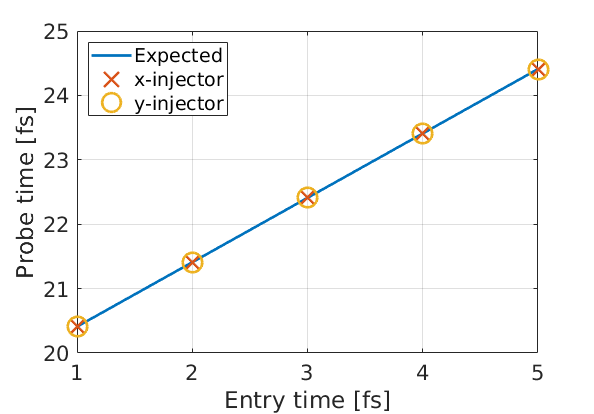
\includegraphics[width=0.6\linewidth]{Figures/bench_file_injector.png}
\caption{Electrons were injected at different times, travelling at 0.86$c$, and probes detected the time they passed the 5 $\mu$m point. For comparison, the solid line is the time we expect electrons to pass the probes, as a function of injection time. Two separate injectors were tested in the same simulation, one injecting from $x_\text{min}$ and the other from $y_\text{min}$}
\label{fig:bench:file_injectors}
\end{figure}

We see excellent agreement between the expected time and the probe time for both injectors. This test was also performed from a restart dump after the 2 fs electrons were injected, and we found our injectors picked up where they left off and injected the correct number of electrons at the correct times. During testing, an issue with the core $\texttt{EPOCH}$ output routines were discovered, as particles inside the simulation window were arriving at the probe at a later time than expected. This was because the particle positions were paired with the wrong time in the SDF file, and were reloaded in the wrong place after the restart (now fixed, see issue \#2229).

\subsubsection{TNSA boundaries} \label{sec:bench:TNSA}

We wrote an input deck to test the three properties of the TNSA boundaries: escaping electrons, reflux momentum loss and reflux scatter, as discussed in Section \ref{sec:code:TNSA}. These were done in hybrid simulations with all the hybrid physics routines switched off. The escape kinetic energy threshold was set to 10 MeV, momentum loss was set to 1 MeV/c, and the scatter angle uncertainty was set to 20$\degree$.

To test all tnsa boundary conditions, we injected two electron bunches, one with a mean kinetic energy of 100 MeV, the other with 5 MeV. All 100 MeV electrons passed through the TNSA boundary, and all 5 MeV electrons reflected with a momentum magnitude change of -$5.341\times 10^{-22}$ kgm$\text{s}^{-1}$ as expected. Figure \ref{fig:bench:tnsa} shows the outgoing angles are uniformly distributed between $\pm 10\degree$, also as expected.

\begin{figure}
\centering
  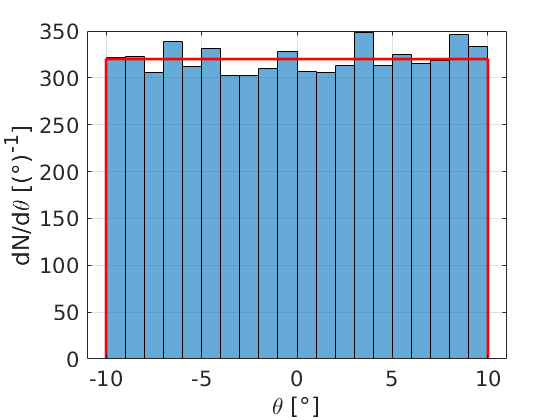
\includegraphics[width=0.6\linewidth]{Figures/bench_tnsa.png}
\caption{Angular distribution of an electron bunch when refluxing through a hybrid TNSA boundary. The solid red line shows the expected distribution, corresponding to a uniform distribution between $\pm 10\degree$.}
\label{fig:bench:tnsa}
\end{figure}

\subsubsection{Thermal equilibration} \label{sec:bench:Equilibration}

We were unable to find experimental data for the temporal evolution of electron and ion temperatures in a solid, so instead we built a simple solver for (\ref{eq:ion_temp}) in \texttt{MATLAB}. This was tested against a hybrid \texttt{EPOCH} simulation, with all hybrid physics switched off apart from thermal equilibration. The electron and ion temperatures were initialised to 100 eV and 50 eV respectively, for an aluminium target. Figure \ref{fig:bench:equilibration} shows the temporal equilibration of temperature for both \texttt{MATLAB} and \texttt{EPOCH}, demonstrating a good agreement between the two codes.

\begin{figure}
\centering
  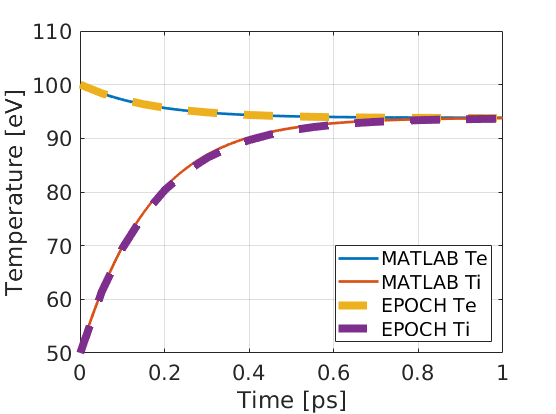
\includegraphics[width=0.6\linewidth]{Figures/bench_equilibration.png}
\caption{Thermal equilibration of the ions and electrons in an aluminium target. The hybrid routines in \texttt{EPOCH} are tested against a \texttt{MATLAB} prototype to demonstrate the hybrid routines are behaving as expected.}
\label{fig:bench:equilibration}
\end{figure}

The ion temperature variable is only treated as a restart variable if it is defined in the code. To ensure it is loaded as expected, this test was also performed in two stages with the code restarting from an output dump in the middle. It was found that the ion temperature was correctly loaded, and the evolution matched that of Figure \ref{fig:bench:equilibration}.

\subsubsection{Geant4 $\delta$-rays} \label{sec:bench:G4_delta}

To test the creation of $\delta$-rays, we injected $10^5$ electrons with kinetic energy 50 keV into an aluminium target. This was simulated in a hybrid simulation, with only ionisation energy loss switched on. While $\delta$-ray emissions down to 1 keV energy were made to affect electron trajectories, only $\delta$-rays above 50 keV energy were added to the simulation. A probe was positioned at 100 $\mu$m to detect passing electrons and $\delta$-rays, and the angular distributions and energy spectra of the particles were recorded. 

This set-up was repeated in \texttt{Geant4}, for simulations where all electromagnetic physics processes were removed from the physics library, except electron ionisation loss. Here, electron and $\delta$-ray momenta were output as they escaped through the rear surface of a 100 $\mu$m aluminium volume. Figure \ref{fig:bench:G4delta}  shows the energy and angular spectra of all electrons (both original and $\delta$-rays) passing the 100 $\mu$m point.

The two codes show good agreement, with most electrons remaining around 50 MeV, with another low energy peak corresponding to the creation of $\delta$-rays. The angular distributions of electrons passing the probe are similar in both codes, but \texttt{EPOCH} over-estimates the large angle scatter. This is because \texttt{Geant4} also considers the binding energy of the $\delta$-ray electron when calculating the energy/momentum conservation (\ref{eq:moller_conservation}). As this is a small effect which mostly affects lower energy electrons, this will be ignored in \texttt{EPOCH}.

\begin{figure}
\centering
\begin{subfigure}{.49\textwidth}
  \centering
  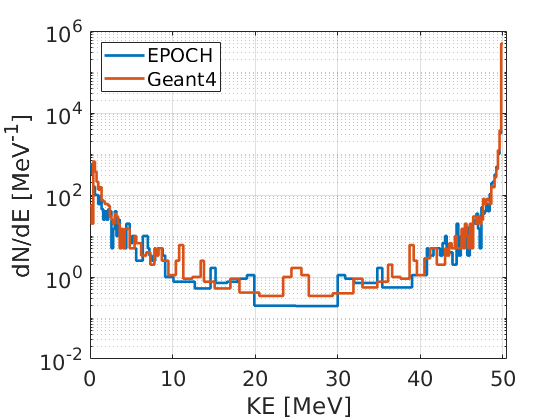
\includegraphics[width=1\linewidth]{Figures/bench_G4delta_E.png}
  \caption{}
\end{subfigure}%
\begin{subfigure}{.49\textwidth}
  \centering
  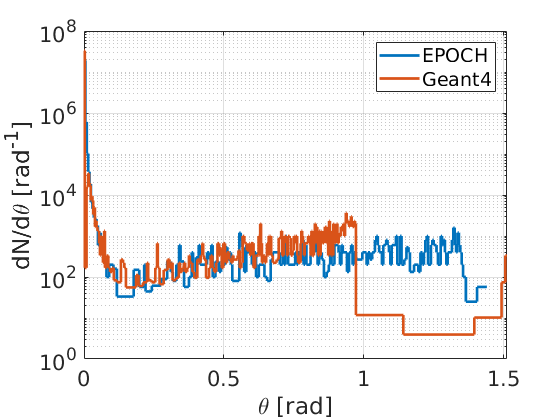
\includegraphics[width=1\linewidth]{Figures/bench_G4delta_ang.png}
  \caption{}
\end{subfigure}
\caption{The energy spectrum (a) and angular distribution (b) of electrons passing 100 $\mu$m in an Al target. The initial bunch consisted of $10^5$ electrons with kinetic energy 50 MeV. Simulations were performed in both \texttt{EPOCH} and \texttt{Geant4}.}
\label{fig:bench:G4delta}
\end{figure}

This test was repeated, split between two runs with a restart in between. This reproduced the original results, which demonstrate the optical depth of $\delta$-ray emission is correctly written to SDF file and reloaded in the restart process.

\subsection{Hanson elastic scatter} \label{sec:bench:Hanson}

Hanson \textit{et al} \cite{benchmark:Hanson} performed an experiment looked at the elastic scatter of 15.7 MeV electrons traversing gold foil targets. This benchmark tests our elastic scatter routines by recreating the experimental electron scatter distribution shown in their Figure 3, for the 18.66 mg/$\text{cm}^2$ (9.67 $\mu$m) target. Two \texttt{EPOCH} input decks were used, both injecting 15.7 MeV (kinetic energy) electron bunches, into gold targets with a particle probe positioned at 9.67 $\mu$m. One input deck used the Davies method for angular scatter, and the other used the Urban method adapted for use in a PIC code. To confirm the validity of our Urban implementation, we also include the result from an equivalent Urban \texttt{Geant4} simulation. The simulation results are shown in Figure \ref{fig:bench:hanson}, along with the Hanson data for comparison.

\begin{figure}
\centering
  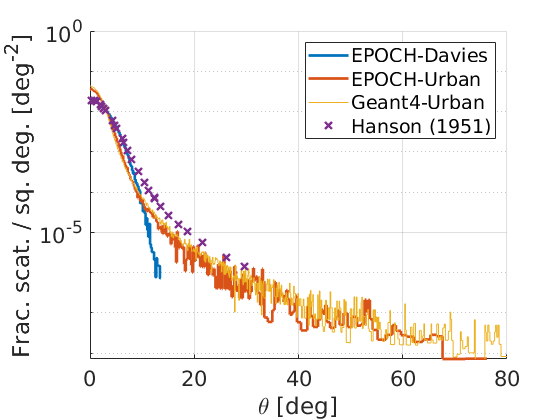
\includegraphics[width=0.6\linewidth]{Figures/bench_Hanson.png}
\caption{The fraction of injected 15.7 MeV electrons passing a particle probe placed 9.67 $\mu$m away from the injection point in a gold target. This number is normalised to the solid angle traced by each $\theta$ bin, in units of square degrees. The experimental data \cite{benchmark:Hanson} is compared against an \texttt{EPOCH} simulation using the Davies method for angular scatter, and \texttt{EPOCH} and \texttt{Geant4} simulations using the Urban method.}
\label{fig:bench:hanson}
\end{figure}

The \texttt{EPOCH} and \texttt{Geant4} Urban curves are in good agreement, which suggest that \texttt{EPOCH} cell sizes are small enough to neglect the difference between geometric and true path lengths using this approach. The Davies algorithm is better at describing small angle scatter, but Urban is better at reproducing the large angle scatter tail (unsurprising as the Urban tail parameters are fit to experimental data). Both curves demonstrate a reasonable agreement with the experimental data for the scatter of most electrons.

\subsection{Lockwood ionisation loss} \label{sec:bench:Lockwood}

This benchmark tests both the angular scatter and continuous ionisation energy loss routines. Lockwood \textit{et al} \cite{benchmark:Lockwood} investigated the energy deposited as a function of target depth for a variety of targets and angles of incidence. Here, we reproduce the depth dose curve for 0.5 MeV electrons in tantalum, as shown in pages 100 and 101 of their report. These simulations injected 0.5 MeV electron bunches, and the deposit energy was inferred from the temperature increase and the known specific heat of tantalum in \texttt{EPOCH}. Figure \ref{fig:bench:lockwood} shows depth-dose curves created using the Davies and Urban algorithms.

\begin{figure}
\centering
  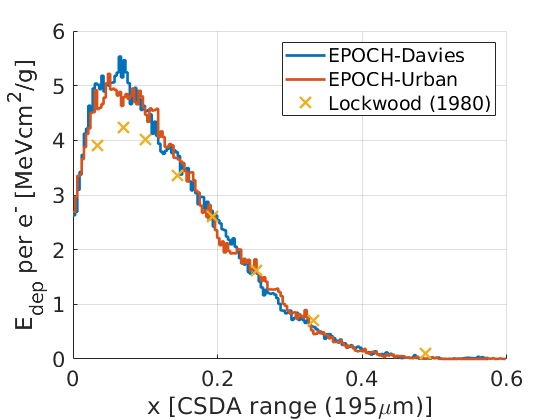
\includegraphics[width=0.6\linewidth]{Figures/bench_Lockwood.png}
\caption{Energy deposition as a function of depth for 0.5 MeV electrons in tantalum. The depth, $x$ is measured in units of expected range of electrons in the material, using the continuous slowing down approximation (CDSA). The energy deposition is quoted as the total energy deposited in MeV per $x$ bin size (cm) per material density (g/$\text{cm}^3$), divided by the total number of incident electrons.}
\label{fig:bench:lockwood}
\end{figure}

This benchmark only tests continuous energy loss, as 0.5 MeV electrons are too low energy to create non-negligible $\delta$-ray or bremsstrahlung X-ray emission. The injected electron current used in the experiment are assumed too small to draw a significant return current. Both algorithms produce good agreement with the experimental data.

\subsection{NIST ionisation and bremsstrahlung} \label{sec:bench:NIST}

In order to test the ionisation and bremsstrahlung energy loss mechanisms for electrons, we repeat the test performed by Wu \textit{et al} \cite{bremPIC:Wu} and measure the total electron stopping power. This benchmark injected several electron bunches at different energies, and calculated their energy loss and step size each step. In order to get a smoother bremsstrahlung curve, the photon weight was reduced to 0.005 (emission 200 times more likely, for bremsstrahlung macro-photons with 0.005 the weight of the emitting macro-electron). The electron stopping powers are shown in Figure \ref{fig:bench:nist} for an Al target, plotted alongside the expected NIST stopping powers \cite{benchmark:Nist}. 

\begin{figure}
\centering
  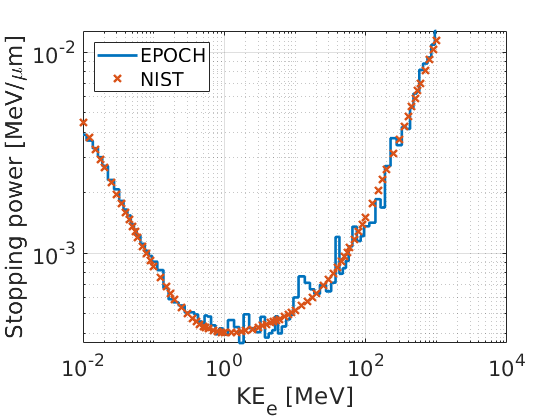
\includegraphics[width=0.6\linewidth]{Figures/bench_NIST.png}
\caption{Stopping power of electrons in Al targets, as a function of the electron kinetic energy.}
\label{fig:bench:nist}
\end{figure}

Figure \ref{fig:bench:nist} shows excellent agreement between \texttt{EPOCH} and NIST, recreating both the ionisation-driven peak at low electron energies, and the high energy bremsstrahlung-driven regime.

\subsection{Milchberg resistivity} \label{sec:bench:Milchberg}

We can test the \texttt{EPOCH} resistivity models by comparing our resistivities against the experimental values found by Milchberg \textit{et al} \cite{eta:Al:Milchberg}. The input deck used for this benchmark set up an aluminium target with no injected electrons, and an initial electron temperature which rose linearly with the $x$ direction. This benchmark tested the reduced Lee-More resistivity model in two simulations, one without any model parameter modification, and other where $\lambda_1$ and $\lambda_2$ have been changed to show better agreement with the data. The resistivity output in each cell was paired with the temperature of that cell to create the curves of Figure \ref{fig:bench:Milchberg}.

\begin{figure}
\centering
  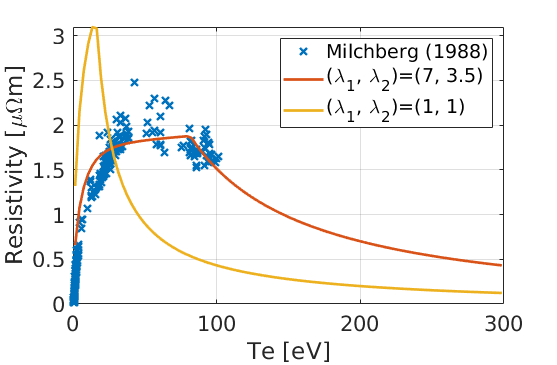
\includegraphics[width=0.6\linewidth]{Figures/bench_milchberg.png}
\caption{Resistivity curves using the reduced Lee-More resistivity model, plotted against the experimental Milchberg data \cite{eta:Al:Milchberg}. The model parameters $\lambda_1$ and $\lambda_2$ have been varied between the two curves, one modified to overlap with the data, the other without any modification.}
\label{fig:bench:Milchberg}
\end{figure}

The model parameter $\lambda_1$ has the effect of causing the peak resistivity to occur at a higher electron temperature, and $\lambda_2$ changes the height of the peak. While the parameterisation allows for greater control over the low temperature side of the resistivity curve, changing $\lambda_2$ from 1 will prevent the high temperature curve reproducing the high temperature limit of the full Lee-More model.

\subsection{Rester bremsstrahlung radiation} \label{sec:bench:Rester}

While Section \ref{sec:bench:NIST} considers the electron energy loss due to bremsstrahlung radiation, the emission of X-rays was not tested. We benchmark X-ray production by reproducing the experimental bremsstrahlung spectra shown by Rester \textit{et al} in their Figure 17 \cite{benchmark:Rester}. This experiment measured the X-ray energy spectrum created when 2.8 MeV electrons passed through a 2.27 g/$\text{cm}^2$ thick (1.176 mm) gold target, for X-rays escaping the target at 10$\degree$, 30$\degree$ and 60$\degree$ to the electron injection direction.

The \texttt{EPOCH} simulations injected electrons of energy 2.8 MeV into a 1.176 mm gold target, and with elastic scatter, ionisation loss and bremsstrahlung switched on. The minimum photon energy added to the simulation was 200 keV, and no bremsstrahlung macro-photon weight modification was used. Bremsstrahlung X-rays within $\pm 5 \degree$ of the Rester angles were grouped, and their energy distributions have been plotted in Figure \ref{fig:bench:rester}.

\begin{figure}
\centering
\begin{subfigure}{.49\textwidth}
  \centering
  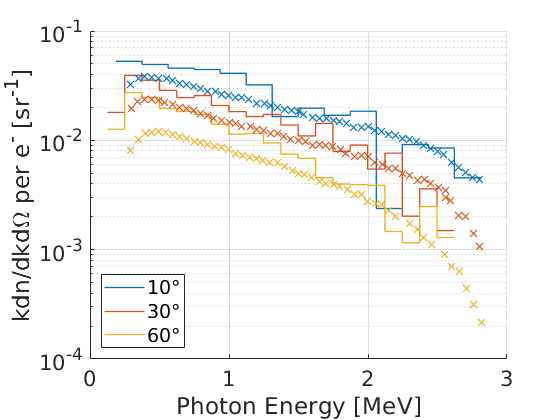
\includegraphics[width=1\linewidth]{Figures/bench_Rester.png}
  \caption{\texttt{EPOCH} vs Rester (1970)}
\end{subfigure}%
\begin{subfigure}{.49\textwidth}
  \centering
  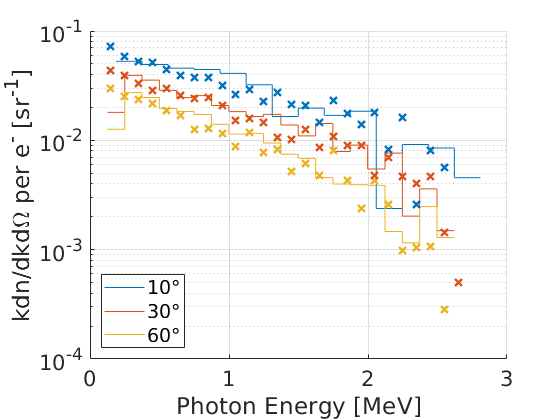
\includegraphics[width=1\linewidth]{Figures/bench_Rester_G4.png}
  \caption{\texttt{EPOCH} vs \texttt{Geant4} without photo-electric effect}
\end{subfigure}
\caption{Energy spectra of bremsstrahlung radiation from 2.8 MeV electrons traversing a 1.176 mm gold target. Bremsstrahlung photons have been grouped by outgoing direction relative to the electron injection axis, $\theta$. The energy spectrum is given as the total X-ray energy in a photon energy bin, divided by the size of the photon energy bin, divided by the total number of injected electrons, divided by the solid angle range of the $\theta$ bin (which spans $\pm 5 \degree$ of the quoted angle for simulated data). The solid line in both figures is the \texttt{EPOCH} data, and the crosses denote the experimental Rester data in (a), and results from a \texttt{Geant4} simulation with all physics switched on apart from the photo-electric effect in (b).}
\label{fig:bench:rester}
\end{figure}

It was found that using angular bremsstrahlung emissions made almost no difference to the angular distribution of X-rays (elastic scatter of electrons dominated). The \texttt{EPOCH} results show generally good agreement with the Rester data, but \texttt{EPOCH} overestimates the low energy X-ray spectra, particularly at higher angles of scatter. This benchmark was repeated in \texttt{Geant4}, and while full \texttt{Geant4} simulations did reproduce the Rester data, we could also reproduce the \texttt{EPOCH} data when switching off attenuation from the photo-electric effect. This effect provides an energy loss mechanism for lower energy X-rays which is not included in \texttt{EPOCH}, and is noticeable in this thick, high-$Z$ target. Hence, \texttt{EPOCH} bremsstrahlung spectra can only be trusted for high energy X-rays, or in thin targets where X-ray attenuation is negligible.

\subsection{Evans background heating} \label{sec:bench:Evans}

This benchmark attempts to recreate the experimental data of Evans \textit{et al} \cite{benchmark:Evans}, which measures the temperature as a function of depth in a target after exposure to a high-intensity short-pulse laser. These 800 fs shots focused 300 J of laser energy into a 10 $\mu$m focal spot, corresponding to a peak intensity of around $3.1\times 10^{20}\text{ Wcm}^{-2}$. Plastic targets were used for this experiment, with a 0.2 $\mu$m Al tracer layer sandwiched at various depths in different targets for experimental temperature measurements. While we can roughly reproduce the laser parameters, we have had to make assumptions on the electron injection angle (set to $20\degree$), and absorption efficiency (set to $3 \%$), hence we are not expecting a perfect fit to the data.

Our simulations use the Davies model for elastic scatter. We use an exponential distribution of injected electrons, with the energy dependent Moore angle also applied. We also use ionisation loss with M\o{}ller scatter, but only add $\delta$-rays over 50 keV kinetic energy to the simulation, otherwise the $\delta$-ray kinetic energy is dumped to the cell for background electron heating. We do not consider thermal equilibration to the ion species, as we are interested in the peak electron temperatures. Bremsstrahlung energy loss and recoil for the electrons is considered, but no X-ray macro-particles are added to the simulation. Perfectly reflective boundaries are used for $x_\text{min}$ and $x_\text{max}$, and the remainder are open (if present). We use the reduced Lee-More model resistivity for Al, with $(\lambda_1,\lambda_2)=(7,3.5)$, and the heuristic plastic resistivity for the plastic targets. The full target in our simulation spans 0 to 32.2 $\mu$m, with the Al tracer layer present between 28 $\mu$m and 28.2 $\mu$m. The temperature distributions are shown in Figure \ref{fig:bench:evans}.

\begin{figure}
\centering
\begin{subfigure}{.49\textwidth}
  \centering
  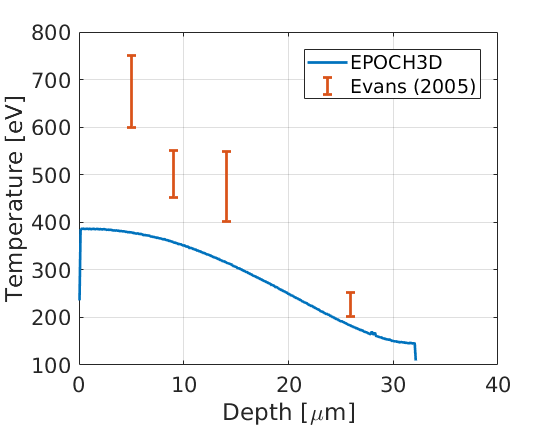
\includegraphics[width=1\linewidth]{Figures/bench_Evans_line.png}
  \caption{}
\end{subfigure}%
\begin{subfigure}{.49\textwidth}
  \centering
  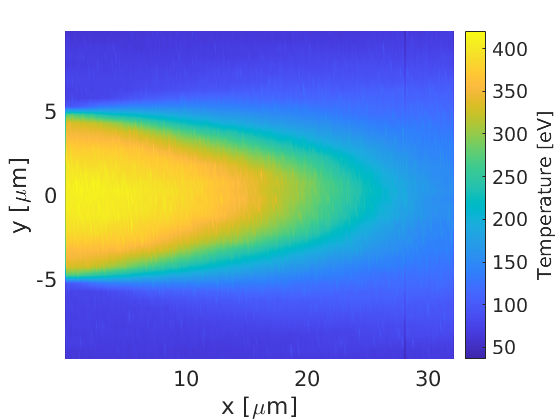
\includegraphics[width=1\linewidth]{Figures/bench_Evans_heat.png}
  \caption{}
\end{subfigure}
\caption{Electron temperature distributions for the CH-Al-CH Evans target after exposure to a 800 fs laser of peak intensity 3.1$\times 10^{22} \text{ Wcm}^{-2}$. We show a line-out of the central temperature (a), and a heatmap of the temperature distribution in the $z=0$ plane for the \texttt{EPOCH3D} result (b).}
\label{fig:bench:evans}
\end{figure}

Given the uncertainty in the absorption parameters, we have a fairly accurate qualitative agreement with the experimental data. The influence of the Al layer can be seen by the slight temperature increase at 28 $\mu$m in Figure \ref{fig:bench:evans}a, and in the line of differing temperatures in Figure \ref{fig:bench:evans}b.

\subsection{Benchmarking summary}

In general, we are capable of reproducing relevant experimental results which demonstrate good agreement with other simulation codes like \texttt{Geant4}. The main inaccuracy revealed in these tests is the lack of the photo-electric effect, which causes \texttt{EPOCH} to overestimate the X-ray spectra of low energy X-rays escaping thick targets. The code also overestimates the large-angle scattering of $\delta$-ray emission, as we do not consider the binding energy of electrons as they are excited. When running \texttt{EPOCH}-hybrid, the user should be aware of these limitations.

\section{User manual} \label{sec:user}

This section aims to provide a general overview of the previous sections, along with information on the new blocks for the \texttt{EPOCH} input deck. See the relevant Theory or Implementation sections for a more detailed breakdown of the codes.

\texttt{EPOCH} now has the capability of running as an electron-transport code for laser-solid simulations. Previously, users interested in simulating laser-solid interactions would have to specify a laser boundary, and represent the solid as a cold, dense collection of macro-particles. This approach is computationally expensive, and prone to unphysical behaviour like numerical self-heating. Electron-transport codes treat the solid as a background static fluid, which a small number of high energy macro-particles move through instead.

To start running these hybrid-PIC simulations, the user must become familiar with three new blocks for the input deck: the \textcolor{blue}{\texttt{hybrid}} block for switching on and off individual subroutines, the \textcolor{blue}{\texttt{solid}} block for defining solid geometries, and the \textcolor{blue}{\texttt{hy\_laser}} block for electron injection. Explanations of these blocks will be provided in the following sections, along with extensions to existing blocks.

\subsection{Hybrid block} \label{sec:user:hybrid}

The hybrid block determines which subroutines are accessed in the hybrid PIC loop, and is also responsible for the initialisation of some background and model parameters. An example hybrid block is shown below:

\begin{lstlisting}[style=myInputDeck]
begin:hybrid

  use_hybrid = T
  use_fields = T
  use_collisions = T
  use_scatter = T
  use_ohmic_heating = T
  use_thomas_fermi = T
  use_ion_temp = F
  produce_delta_rays = T
  electron_temperature = 300 
  ion_temperature = 300      
  min_delta_KE = 50.0*kev
  min_hybrid_KE = 1.0*ev
  elastic_model = Davies
  rlm_1 = 1
  rlm_2 = 1         

end:hybrid
\end{lstlisting}

\bigskip {\large\textcolor{blue}{use\_hybrid}} - Logical flag to determine if we use the hybrid PIC loop. This must be set to T if the code is to run in hybrid mode. The default is F.

\bigskip {\large\textcolor{blue}{use\_fields}} - Logical flag to switch on the hybrid field solver (default F). If T, the electric and magnetic fields will be updated assuming a return current is drawn from the solid background, otherwise fields will remain at their initial values.

\bigskip {\large\textcolor{blue}{use\_scatter}} - Logical flag to switch on elastic scatter routines for incoming electrons. The default is F (no elastic scatter).

\bigskip {\large\textcolor{blue}{elastic\_model}} - Choose the elastic scatter algorithm to use. The options are \textcolor{blue}{\texttt{Davies}} or \textcolor{blue}{\texttt{Urban}}. Davies is more accurate for small angle scatter and faster to run, while Urban is more appropriate if you are interested in rarer large-angle scatter events. The default is Davies.

\bigskip {\large\textcolor{blue}{use\_collisions}} - Logical flag to switch on ionisation energy loss routines. This is the energy loss from incident electrons due to exciting the atomic electrons in the background solid. The default is F (no ionisation energy loss).

\bigskip {\large\textcolor{blue}{produce\_delta\_rays}} - In ionisation energy loss, incident electrons can lose a lot of energy to atomic electrons, exciting them into secondary high-energy electrons (termed $\delta$-rays). Ionisation energy loss routines will always calculate the incident electron recoil due to $\delta$-ray emission, but will only add them to the simulation window if this key is T. Otherwise, the $\delta$-ray energy is used to raise the local background electron temperature. The default is F.

\bigskip {\large\textcolor{blue}{min\_delta\_energy}} - Minimum $\delta$-ray total energy to be injected into the simulation [J]. \textcolor{blue}{produce\_delta\_rays} must be T to inject any $\delta$-rays at all. The default is $m_e c^2$ (all $\delta$-rays added, very slow).

\bigskip {\large\textcolor{blue}{min\_delta\_KE}} - Sets the same parameter as \textcolor{blue}{min\_delta\_energy}, but using the minimum kinetic energy instead [J]. Default is 0 (all $\delta$-rays added, very slow).

\bigskip {\large\textcolor{blue}{min\_hybrid\_energy}} - Sets the minimum electron energy in allowed in the simulation window [J]. Any electrons below this energy are removed from the simulation, and their energy is dumped into a background electron temperature increase. Due to the heating aspect, this currently requires ionisation energy loss to be switched on in order to work. Default is $m_e c^2$ (only remove electrons at rest).

\bigskip {\large\textcolor{blue}{min\_hybrid\_KE}} - Sets the same parameter as \textcolor{blue}{min\_hybrid\_energy}, but using the minimum kinetic energy instead [J]. Default is 0 (only remove electrons at rest).

\bigskip {\large\textcolor{blue}{use\_ohmic\_heating}} - Logical switch to use Ohmic heating. This involves a background electron temperature increase in each step, based on the local resistivity and hot electron current density. The default is F (no heating).

\bigskip {\large\textcolor{blue}{use\_thomas\_fermi}} - Logical switch to calculate the ionisation state of the background solid, using a fit to the Thomas-Fermi distribution. The default is F (no ionisation calculation), but this can be overwritten by routines which require ionisation like the reduced Lee-More resistivity model, or bremsstrahlung radiation with plasma screening switched on.

\bigskip {\large\textcolor{blue}{use\_ion\_temp}} - Logical switch to use the ion-electron thermal equilibration routines, which exchange heat between the two particle species. The default is F (no heat exchange).

\bigskip {\large\textcolor{blue}{electron\_temperature}} - Initial background electron temperature distribution, which can vary in space (Kelvin). Default is 0 in all cells.

\bigskip {\large\textcolor{blue}{ion\_temperature}} - Initial background ion temperature distribution, which can vary in space (Kelvin). Default is 0 in all cells.

\bigskip {\large\textcolor{blue}{rlm\_1}} - The $\lambda_1$ parameter used in the reduced Lee-More resistivity model. The default is 7 to match the Milchberg curve.

\bigskip {\large\textcolor{blue}{rlm\_2}} - The $\lambda_2$ parameter used in the reduced Lee-More resistivity model. The default is 3.5 to match the Milchberg curve.

\subsection{Solid block} \label{sec:user:solid}

To specify the solid geometries in the hybrid routines, a special solid block has been developed. Solids can be positioned by specifying the ion number density over the simulation window. A solid may only represent one element, but compound materials like plastic can be built by spatially overlapping a carbon and a hydrogen solid. An example solid block is shown below for an Al solid positioned between $x=0$ and $x=10$ $\mu$m

\begin{lstlisting}[style=myInputDeck]
begin:solid

  atomic_no = 13
  mass_no = 27
  I_ex = 166 * ev
  ni = if ((x gt 0) and (x lt 10), 6.022e28, 0)
  rad_len = 0.08897
  resistivity = rlm

end:solid
\end{lstlisting}

\bigskip {\large\textcolor{blue}{atomic\_no}} - Atomic number of the solid (integer).

\bigskip {\large\textcolor{blue}{mass\_no}} - Mass number of the solid.

\bigskip {\large\textcolor{blue}{I\_ex}} - Mean excitation energy of the solid or compound solid.

\bigskip {\large\textcolor{blue}{ni}} - Ion number density of the solid.

\bigskip {\large\textcolor{blue}{rad\_len}} - Radiation length of the solid or compound solid (only required if using Urban elastic scatter). The radiation length assigned to each cell will match the radiation length of the solid with the highest background electron number density in this cell at the time of initialisation.

\bigskip {\large\textcolor{blue}{resistivity}} - Resistivity model for electrons in this solid or compound solid. The resistivity model used will match the resistivity model of the solid with the highest background electron number density in this cell at the time of initialisation. Options are \textcolor{blue}{\texttt{rlm}}, \textcolor{blue}{\texttt{Milchberg}}, \textcolor{blue}{\texttt{plastic}} or \textcolor{blue}{\texttt{vacuum}}. 

\subsection{Hybrid laser block} \label{sec:user:hy_laser}

When working with hybrid routines, it is useful to have a way to inject electrons which is more general than the Maxwellian injector already present in the code. The \textcolor{blue}{\texttt{hy\_laser}} block was designed to produce expected electron distributions based on laser parameters, such that the block shares many keys with a standard laser block (despite being a particle injector). This block is also capable of injecting particle beams and bunches, at a variety of angles using multiple models. For details on the mean energy, particle energy and angular distribution models, consult Section \ref{sec:code:injector} and its various subsections. Here we restrict our discussion to the keys in the input deck. When discussing angles, we define $\theta$ as an angle to the boundary normal, and $\phi$ as an azimuthal rotation about the normal. An example \textcolor{blue}{\texttt{hy\_laser}} block is shown below:

\begin{lstlisting}[style=myInputDeck]
begin:hy_laser

  boundary = x_min
  ppc = 5
  profile = gauss(y,0,5.0e-6)*gauss(z,0,5.0e-6)
  profile_min = 0.5

  t_profile = gauss(time, 730.0e-15, 340.0e-15)
  t_start = 0.0
  t_end = 1460.0e-15

  intensity = 3.1e20 * 1.0e4
  lambda = 1.0e-6
  efficiency = 0.03 

  mean_energy = a0
  energy_dist = exp_weight
  angular_dist = uniform

  theta_max = 20.0/180.0*pi
  mean_mult = 10.0
  use_moore_max = T

  species = Electron

end:hy_laser
\end{lstlisting}

\bigskip {\large\textcolor{blue}{boundary}} - Boundary of particle injection, can be \textcolor{blue}{\texttt{x\_min}} or \textcolor{blue}{\texttt{x\_max}}, or higher dimensions in \texttt{EPOCH2D} and \texttt{EPOCH3D}.

\bigskip {\large\textcolor{blue}{ppc}} - If a cell injects particles this time step, this key specifies how many macro-particles to inject.

\bigskip {\large\textcolor{blue}{omega}} - Laser angular frequency. If using laser-based injection, specify this, frequency or wavelength. Can be a function of time.

\bigskip {\large\textcolor{blue}{frequency}} - Laser frequency. If using laser-based injection, specify this, angular frequency or wavelength. Can be a function of time.

\bigskip {\large\textcolor{blue}{wavelength}} - Laser wavelength. If using laser-based injection, specify this, frequency or angular frequency. Can be a function of time.

\bigskip {\large\textcolor{blue}{intensity}} - Peak cycle-averaged laser intensity.

\bigskip {\large\textcolor{blue}{efficiency}} - Conversion efficiency of laser energy into particle kinetic energy, for determining the weights of macro-particles

\bigskip {\large\textcolor{blue}{profile}} - Spatial profile of the laser pulse. Must be less than or equal to 1 at all points, otherwise laser intensity will exceed the peak value given by the \textcolor{blue}{\texttt{intensity}} key.

\bigskip {\large\textcolor{blue}{profile\_min}} - If the spatial profile dips below this number, no particles will be added in that cell.       

\bigskip {\large\textcolor{blue}{t\_profile}} - Temporal profile of the laser pulse. Must be less than or equal to 1 at all points, otherwise laser intensity will exceed the peak value given by the \textcolor{blue}{\texttt{intensity}} key.

\bigskip {\large\textcolor{blue}{t\_start}} - Time at which particles can start to be injected.

\bigskip {\large\textcolor{blue}{t\_end}} - No particles will be injected after this time.

\bigskip {\large\textcolor{blue}{species}} - Particle species to populate with injected particles.

\bigskip {\large\textcolor{blue}{mean\_energy}} - Model for calculating the mean injected particle energy. Options are: \textcolor{blue}{\texttt{a\_0}} ($a_0 m_e c^2$) or \textcolor{blue}{\texttt{Wilks}} for laser-based mean energies, or \textcolor{blue}{\texttt{E\_val}} for a user-defined mean energy.

\bigskip {\large\textcolor{blue}{mean\_E}} - User-defined mean total particle energy for the \textcolor{blue}{\texttt{E\_val}} mean energy model. Specify this or \textcolor{blue}{\texttt{mean\_KE}}.

\bigskip {\large\textcolor{blue}{mean\_KE}} - User-defined mean particle kinetic energy for the \textcolor{blue}{\texttt{E\_val}} mean energy model. Specify this or \textcolor{blue}{\texttt{mean\_E}}.

\bigskip {\large\textcolor{blue}{energy\_dist}} - Model for calculating the energy and weight distributions of injected macro-particles. All weights are uniform and calculated from laser parameters unless otherwise stated. The options are: \textcolor{blue}{\texttt{exp}} (exponential energy distribution), \textcolor{blue}{\texttt{mono}} (mono-energetic at mean energy), \textcolor{blue}{\texttt{top\_hat}} (uniform energy between two limits), \textcolor{blue}{\texttt{exp\_weight}} (uniform energies, exponential weights), \textcolor{blue}{\texttt{mono\_weight}} (mono-energetic with user-defined weight), and \textcolor{blue}{\texttt{mono\_las\_weight}} (mono-energetic, but particle energies can be different from mean energy calculation).

\bigskip {\large\textcolor{blue}{mono\_weight}} - User-defined particle weights for the \textcolor{blue}{\texttt{mono\_weight}} energy distribution model.

\bigskip {\large\textcolor{blue}{las\_weight\_KE}} - User-defined particle energy for the \textcolor{blue}{\texttt{mono\_las\_weight}} energy distribution model. Useful if you don't want to inject particles with the same mean energy as that used to calculate the laser injection weights.

\bigskip {\large\textcolor{blue}{top\_hat\_L}} - Width of the uniform distribution for the \textcolor{blue}{\texttt{top\_hat}} energy distribution model. Particles are injected between $\pm$ this fraction of the mean kinetic energy.

\bigskip {\large\textcolor{blue}{mean\_mult}} - Maximum energy modelled by the \textcolor{blue}{\texttt{exp\_weight}} distribution, expressed as a multiplication factor applied to the mean kinetic energy.

\bigskip {\large\textcolor{blue}{angular\_dist}} - Model for calculating the angular distribution of injected macro-particles. Options are: \textcolor{blue}{\texttt{uniform}} (isotropic), \textcolor{blue}{\texttt{cos}} ($\propto \cos^n(\theta)$), \textcolor{blue}{\texttt{beam}} (all particles same direction).

\bigskip {\large\textcolor{blue}{cos\_n\_power}} - The value of $n$ in $\cos^{n}(\theta)$ for the \textcolor{blue}{\texttt{cos}} angular distribution model. 

\bigskip {\large\textcolor{blue}{theta\_max}} - Maximum $\theta$ value for injected particles.

\bigskip {\large\textcolor{blue}{use\_moore\_max}} - Logical switch to use Moore scaling on the injected particle angle. This is an energy dependent maximum $\theta$, and particles will be given angles up to the Moore angle or \textcolor{blue}{\texttt{theta\_max}}, whichever is lower.    

\bigskip {\large\textcolor{blue}{use\_sheng\_dir}} - Logical switch to use the energy-dependent Sheng injection angle for oblique laser pulses.

\bigskip {\large\textcolor{blue}{sheng\_angle}} - The angle the laser makes to the target normal, a parameter for the Sheng model.

\bigskip {\large\textcolor{blue}{theta}} - Global $\theta$ rotation of the injected particles after all angular distribution models have been applied.

\bigskip {\large\textcolor{blue}{phi}} - Global $\phi$ rotation of the injected particles after all angular distribution models have been applied. The meaning of $\phi=0$ and the direction of increasing $\phi$ has different meanings on different boundaries. On boundaries \{$x_\text{min}$, $x_\text{max}$, $y_\text{min}$, $y_\text{max}$, $z_\text{min}$, $z_\text{max}$\}, the $\phi=0$ line points to \{$z_\text{min}$, $z_\text{min}$, $z_\text{min}$, $z_\text{min}$, $x_\text{max}$, $x_\text{max}$\}, and the direction of increasing $\phi$ makes $\phi=\pi/2$ point towards \{$y_\text{max}$, $y_\text{min}$, $x_\text{min}$, $x_\text{max}$, $y_\text{max}$, $y_\text{max}$\}.      

\subsection{Hybrid keys in existing blocks} \label{sec:user:extra}

Finally, some new hybrid functionality is present in existing input deck blocks. The remainder of this section will cover these new extensions.

\subsubsection{TNSA boundary}

We have implemented a new type of boundary condition to mimic the behaviour of electrons refluxing in the sheath field. This involves allowing high energy electrons to escape, while reflecting lower energy electrons with some momentum loss and scatter. An example block with TNSA boundaries is given below:

\begin{lstlisting}[style=myInputDeck]
begin:boundaries

  bc_x_min = tnsa
  bc_x_max = tnsa
  bc_y_min = reflect
  bc_y_max = reflect
  bc_z_min = reflect
  bc_z_max = reflect

  tnsa_escape_KE = 10e6 * ev
  tnsa_p_loss = 5.341e-22
  tnsa_scatter_deg = 20     

end:boundaries
\end{lstlisting}

The TNSA keys are currently shared between all boundaries with TNSA boundary conditions. A breakdown of these new keys is provided here:

\bigskip {\large\textcolor{blue}{tnsa\_escape\_KE}} - TNSA boundaries are reflective, but particles above this kinetic energy will not be reflected and escape the simulation window.

\bigskip {\large\textcolor{blue}{tnsa\_p\_loss}} - Reflecting particles will have their momentum magnitude reduced by this amount on tnsa boundaries (or set to zero if their momentum is too low).

\bigskip {\large\textcolor{blue}{tnsa\_scatter\_angle}} - The $\theta$ angle of reflecting particles will be changed by a number drawn from a uniform distribution between $\pm$ the value of this key, in radians.

\bigskip {\large\textcolor{blue}{tnsa\_scatter\_deg}} - Same as \textcolor{blue}{tnsa\_scatter\_angle}, but in degrees.

\subsubsection{Hybrid output variables}

The hybrid routines introduce a new particle variable which can be written to SDF files from the output block:
\\
\\
\indent\bigskip {\large\textcolor{blue}{delta\_optical\_depth}} - The optical depths associated with emission of a $\delta$-ray.
\\
We also have 5 new field variables to output properties of the hybrid solid background:
\\
\\
\indent\bigskip {\large\textcolor{blue}{hy\_Te}} - Background electron temperature (Kelvin).
\\
\indent\bigskip {\large\textcolor{blue}{hy\_Ti}} - Background ion temperature (Kelvin).
\\
\indent\bigskip {\large\textcolor{blue}{hy\_ni}} - Background ion number density.
\\
\indent\bigskip {\large\textcolor{blue}{hy\_ion\_charge}} - Background average ion charge state (from Thomas-Fermi ionisation).
\\
\indent\bigskip {\large\textcolor{blue}{hy\_resistivity}} - Resistivity of the background solids.
\\
The optical depth and electron temperature are restart variables, and ion temperature is only a restart variable if it has been allocated in the code.

\subsubsection{File injector}

The injector block has been extended to now inject particles defined in files. Ensure each particle variable is given its own file, and particles are ordered by injection time. An example block is provided below:

\begin{lstlisting}[style=myInputDeck]
begin:injector

  boundary = x_min
  species = Electron
  
  inject_from_file = T 
  
  y_data = "../injectors/y.txt"
  z_data = "../injectors/z.txt"
  px_data = "../injectors/px.txt"
  w_data = "../injectors/w.txt"
  t_data = "../injectors/t.txt"
  id_data = "../injectors/id.txt"

end:injector
\end{lstlisting}

\bigskip {\large\textcolor{blue}{inject\_from\_file}} - Override normal injector block routines and inject particles from file.

\bigskip {\large\textcolor{blue}{\texttt{\{...\}\_data}} - The path to the file containing a list of variable values for injecting particles. In higher dimension \texttt{EPOCH} versions we can define the injection position with \textcolor{blue}{\texttt{x\_data}}, \textcolor{blue}{\texttt{y\_data}} and \textcolor{blue}{\texttt{z\_data}} if appropriate. Injection momentum is set using \textcolor{blue}{\texttt{px\_data}}, \textcolor{blue}{\texttt{py\_data}} and \textcolor{blue}{\texttt{pz\_data}} (assumed 0 if omitted). The weight of injected particles is given by the \textcolor{blue}{\texttt{w\_data}} file, the injection times are given by \textcolor{blue}{\texttt{t\_data}} and we can assign particle IDs to injected particles using \textcolor{blue}{\texttt{id\_data}}.

\bibliographystyle{unsrt}
\bibliography{hybrid_documentation_bib.bib}

\end{document}
